\documentclass[authoryear]{article}
\usepackage{amsmath}
\usepackage{amssymb}
\usepackage{array}
\usepackage{bm}
\usepackage{epsfig}
\usepackage{graphicx}
\usepackage{geometry}
\usepackage{gensymb}
\usepackage{moresize}
%\usepackage[round]{natbib}
\usepackage{natbib}
\usepackage{pifont}
\usepackage{rotating}
\usepackage{url}

\geometry{dvips,paperwidth=8.5in,paperheight=11in,body={6.5in,9.5in},left=1in,
top=1in}
\widowpenalty=1000 \clubpenalty=1000
\renewcommand{\baselinestretch}{1.25}


%%This code prevents big figures from being 
 % See p.105 of "TeX Unbound" for suggested values.
    % See pp. 199-200 of Lamport's "LaTeX" book for details.
    %   General parameters, for ALL pages:
    \renewcommand{\topfraction}{0.9}	% max fraction of floats at top
    \renewcommand{\bottomfraction}{0.8}	% max fraction of floats at bottom
    %   Parameters for TEXT pages (not float pages):
    \setcounter{topnumber}{2}
    \setcounter{bottomnumber}{2}
    \setcounter{totalnumber}{4}     % 2 may work better
    \setcounter{dbltopnumber}{2}    % for 2-column pages
    \renewcommand{\dbltopfraction}{0.9}	% fit big float above 2-col. text
    \renewcommand{\textfraction}{0.07}	% allow minimal text w. figs
    %   Parameters for FLOAT pages (not text pages):
    \renewcommand{\floatpagefraction}{0.7}	% require fuller float pages
	% N.B.: floatpagefraction MUST be less than topfraction !!
    \renewcommand{\dblfloatpagefraction}{0.7}	% require fuller float pages

% Set up the images/graphics package
\setkeys{Gin}{width=\linewidth,totalheight=\textheight,keepaspectratio}
\graphicspath{{graphics/}}

% The following package makes prettier tables.  We're all about the bling!
\usepackage{booktabs}

% The units package provides nice, non-stacked fractions and better spacing
% for units.
\usepackage{units}

% The fancyvrb package lets us customize the formatting of verbatim
% environments.  We use a slightly smaller font.
\usepackage{fancyvrb}
\fvset{fontsize=\normalsize}

% Small sections of multiple columns
\usepackage{multicol}

% Provides paragraphs of dummy text
\usepackage{lipsum}

% Allows within line comments for editing 
\usepackage{comment}

% These commands are used to pretty-print LaTeX commands
\newcommand{\doccmd}[1]{\texttt{\textbackslash#1}}% command name -- adds backslash automatically
\newcommand{\docopt}[1]{\ensuremath{\langle}\textrm{\textit{#1}}\ensuremath{\rangle}}% optional command argument
\newcommand{\docarg}[1]{\textrm{\textit{#1}}}% (required) command argument
\newenvironment{docspec}{\begin{quote}\noindent}{\end{quote}}% command specification environment
\newcommand{\docenv}[1]{\textsf{#1}}% environment name
\newcommand{\docpkg}[1]{\texttt{#1}}% package name
\newcommand{\doccls}[1]{\texttt{#1}}% document class name
\newcommand{\docclsopt}[1]{\texttt{#1}}% document class option name
%Prints a degree symbol
\newcommand{\degreesym}{\ensuremath{^\circ}}



\begin{document}
\title{Supporting the Development of Direct Climate Markets: Pricing Uncertainty in ENSO Forecasts}
\date{}  % if the \date{} command is left out, the current date will be used
%
%\author[grant]{Grant Cavanaugh}
%
%\author[wharton]{Benjamin L. Collier}
%\ead{bencol@wharton.upenn.edu}
%
%\author[uky]{Jerry R. Skees}
%\ead{jerry.skees@uky.edu}
%
%\address[grant]{Cavanaugh LLC}
%\address[wharton]{Wharton Risk Management and Decision Processes Center, University of Pennsylvania, Phialdelphia, PA 19104, USA}
%\address[uky]{Department of Agricultural Economics, University of Kentucky, Lexington, KY 40546, USA}
%


\maketitle% this prints the handout title, author, and date
\begin{abstract}
This paper discusses how financial markets for indexes of regional climate anomalies with long-range physical and statistical links to extreme weather events, or what climate scientists call \emph{teleconnections}, might address that market gap. It suggests that the social gains from these markets would be particularly high if they included active trading. To that end, it provides tools necessary to incubate risk trading for the best known teleconnection, El Ni\~no-Southern Oscillation (ENSO).
\end{abstract}

\section{Introduction}
Existing financial and insurance markets fail to provide protection against, and clear forecasts of, climate risk. There are many markets today where firms and individuals can trade or manage risk influenced by climate. Among the better known are traded markets for emission permits, temperature and rainfall derivatives for major cities, and equities for companies in weather dependent industries. Similarly, there are markets for insurance and reinsurance risks traded by specialized institutional investors \citep{kurtov2010investing}[INSERT CHAPTER SPECIFIC REF]. But none of these markets offer at-risk communities direct protection from climate extremes at competitive prices – prices that represent an informed forecast of global weather patterns. Instead, prices on these markets are primarily driven by non-climate factors like policy and recent returns in bond and equity markets \citep{econ2013ETS} \citep{kurtov2010investing}[INSERT CHAPTER SPECIFIC REF]. This discrepancy - between a risk as it is experienced by individuals and the index underlying a market where individuals are supposed to manage that risk - is an example of what is called in finance \emph{high basis risk}.

One alternative to existing markets could be markets based on basic indexes of climate change, like the extent of Arctic ice or global mean surface temperatures. But, meaningful shifts in these indexes, if they occur as seem likely according to current climate models, will play out over long-time horizons \cite{ipcc2013fifthReport}. Those horizons complicate collective decision making in particular, but they also pose a challenge to individual economic experts evaluating the merits of hedging climate risk \cite{jacquet2013intra} \cite{nordhaus2013}[Need SPECIFIC CHAPTER REF OR PAPER REF] \cite{pindyck2013}. Moreover, the models used to simulate global climate change have not progressed to the point where they can translate those global indexes into forecasts of adverse climate events on a geographic scale that is actionable for many firms [Need SPECIFIC CITATION PERHAPS IPCC ON LIMITATIONS OF GLOBAL MODELS]. In this case, an actionable geographic scale would be one focused enough to convince risk managers that a climate risk would imperil specific contractual relationships, a key factor motivating hedging \cite{pennings2000motivation} \cite{pennings2001behavioural}. Hence, it is not clear that there is latent demand for hedges against the indexes that have come to define global climate change.

Together, the difficulties of building meaningful financial contracts directly around climate change and the basis risk inherent to managing climate risk with existing markets suggest a missing market, one that could:

\begin{itemize}
\item Directly cover climate risks more pervasive than simple short-term weather indicators;
\item Meet conditions associated with stable financial risk transfer flows \cite{working1953futures} \cite{silber1981innovation} \cite{carlton1984futures} \cite{black1986success} \cite{duffie1989optimal} \cite{tashjian1995optimal} \cite{pennings1999commodity} \cite{brorsen2001success} \cite{gorham12} \cite{sandor2012}; and
\item Fit within the actionable geographic scope and time horizons of decision makers attempting to prepare for a changing climate. 
\end{itemize}

This paper discusses how financial markets for indexes of regional climate anomalies with long-range physical and statistical links to extreme weather events, or what climate scientists call \emph{teleconnections}, might address that market gap. It suggests that the social gains from these markets would be particularly high if they included active trading. To that end, we provide a framework for thinking about traded teleconnection index risk and tools necessary to incubate risk trading for the best known teleconnection index, El Ni\~no-Southern Oscillation (ENSO). [BEN I DON'T THINK YOU LIKE CALLING THIS TOOLS. CAN YOU HELP ME REPHRASE THIS WITHOUT GETTING JARGONY] 

Although most of the analysis presented here is focused on ENSO, it addresses questions that are broadly applicable to risk markets that might come to sit at the intersection of finance and science such as When is a scientific risk well suited to direct management on a traded market? How can a new science-driven risk market avoid the asymmetric information problems that could undermine active trading? When do scientific forecasts contain financially actionable information? How can we incorporate multiple sources of scientific uncertainty into risk markets? Does a new risk show enough volatility to sustain active trading? 

El Ni\~no-Southern Oscillation (ENSO) (more specifically the Oscillation's extreme anomaly events called El Ni\~no/La Ni\~na) is a climate driver with teleconnections whose risk is already directly managed through an innovative insurance that the authors helped design, and facilitate sales of, with support from the Gate Foundation. This emerging El Ni\~no insurance market is noteworthy in that it is the first market to directly hedge teleconnection risk and has been structured as forecast insurance - an insurance that pays based on a remotely measured geophysical event that precedes much of El Ni\~no's physical damage. 

The nascent market for El Ni\~no insurance suggests a greater potential to transfer teleconnection risks around the world. Traded risk management tools based on existing El Ni\~no insurance, but relevant to ENSO hedgers across the globe, may the best opportunity to provide at-risk communities with an actionable risk management tool that could be the basis of climate risk adaptation strategies [SHOULD THIS BE MITIGATION?] and that generates prices whose climate forecast information is of wide social value. ENSO and other indexes with teleconnections directly causing extreme weather in specific communities. Hence these climate drivers are specific enough to worry individuals, firms, and institutions in the short-term. Yet, they are also long-dated and wide-ranging phenomenon, clearly linked to global climate change. 

In this article we introduce practical considerations for the development of such markets. We discuss the nature of ENSO risk and why that risk may generate high social welfare gains if it were managed on traded markets. Then, we introduce a pricing framework that is necessary but not sufficient to catalyze early trades those markets. This framework will give benchmark prices to risk managers seeking climate protection, even as new forecast information becomes available. Dealing with such forecast information and placing a price on the uncertainty within that information is a critical hurdle for the development of robust direct climate markets. Indeed the information asymmetries associated with ENSO forecasts have complicated the sale of existing insurance against extreme El Ni\~no in Peru, which we helped design and sell with support from the Gates Foundation. 

In addition, to providing a starting point for risk transfer negotiations our pricing framework helps to answer questions of importance to the financial firms that might allocate resources to trading on direct climate markets, such as whether information about extreme ENSO events changes sufficiently to warrant active trading.

\subsection{Introduction to ENSO risk}
ENSO refers to a coupled oceanic/atmospheric cycle. In normal years, the cycle follows currents and winds (each reinforcing the other) as they bring water along the surface of the Pacific Ocean from South America (the eastern side of the Pacific) to Indonesian and the South Pacific (the western side of the Pacific). As that water travels along the ocean surface, it warms. The resulting mass of warm water sinks as it arrives in the western Pacific and begins circulating back toward Peru along the cold ocean floor. The cycle ends with cold water rising to the surface in the eastern Pacific, sustaining rich fishing grounds off the coast of Peru and Chile.

During an El Ni\~no anomaly, this cycle weakens. Usually starting in March or April, a plume of warmer-than-normal water creeps eastward across the Pacific, lessening the normal temperature gradient from the Western to the Eastern Pacific. When that plume of warmer-than-normal water reaches Peru, it parks a moisture laden air mass off the South American coast. When that mass meets cold air coming east to west over the Andes mountains, Peru suffers catastrophic downpours and flooding. Those rains generally arrive in the early months of the year following the initial warming.

By contrast, during a La Ni\~na anomaly the normal cycle enhances. More water gets pushed from the South American coast, raising sea-surface temperatures in Australia and Indonesia above normal. That leaves Southeast Asia and Oceania with increased incidence of extreme rains and flooding.

\subsubsection{ENSO Risk Characteristics and the Limitations of ENSO Insurance}
The physical risk of El Ni\~no/La Ni\~na includes characteristics that are important from the standpoint of risk management. These characteristics allowed GlobalAgRisk to create an innovative El Ni\~no insurance. However, they also suggest why, eventually, ENSO risk may be better managed through traded markets. These characteristics include:
\begin{itemize}
\item ENSO anomalies are measured by a relatively simple index.
National Meteorological Services (NMS) monitor El Ni\~no/La Ni\~na primarily by measuring sea-surface temperatures (SST) over defined regions of the Pacific Ocean. That means that the the phenomenon can be accurately expressed using freely available data, provided in simple-to-understand units, according to a methodology that is well defined. These qualities are attractive to prospective speculators (those offering El Ni\~no protection in exchange for an expected profit), because they mitigate many of the moral hazard and adverse selection problems inherent to traditional insurance. [INCLUDE JERRY CITATION] 
% Also, the simplicity and reliability of the data lowers the cost of underwriting protection. Most catastrophic risks are inherently multi-variate. Hurricanes for example, even in an indexed form, require estimates of windspeeds, storm track, and the time that a storm will spend over a given area. This is sufficiently complicated that even sophisticated hedge funds specializing in catastrophic risk effectively outsource much of their underwriting by licensing catastrophe models from firms like RMS and AIR Worldwide that employ large teams of climate scientists. By contrast, monthly SST are univariate timeseries. 
\item Anomalies in SSTs translate to discrete risk outcomes that are well understood by at-risk communities.
Speculators' preference for simple and reliable indexes are not enough to drive a new insurance market. The indexes must correspond tightly to hedgers/insurance buyers' risk perceptions.[WORKING? DUFFIE? CUNY? TASHJIAN?] That is indeed the case for NOAA's SST indexes. 

Perceived basis risk is particularly low for Peruvian hedgers managing the risk of catastrophic flooding in the country's Northern region using SST measurements from the Ni\~no 1.2 region, directly off the Peruvian coast. In fact, the high SSTs measured by NOAA's various indexes are the immediate physical cause of flooding, so the link between the index and risk outcomes is more a simple statistical association\cite{khalil2007nino}. 

Rainfall in northern Peru during the last severe El Ni\~no in 1998 was 40 times normal for January to May \citep{skees2009enso}. This event caused widescale internal displacement of people; loss of life; increases water-born illnesses; disruptions to markets and supply chains; and destruction of personal property and critical infrastructure. There were similarly headline-grabbing impacts from the 1983 El Ni\~no.

Both of those years standout from the rest in Ni\~no SST time series covering the critical months between October and January. This is clear in figure [INSERT FIGURE] which shows the November/December average SSTs for NOAA's Ni\~no 1.2 region, which GlobalAgRisk used as the base index of it's insurance.

The spikes in that index correspond so well to the years popularly associated with catastrophic El Ni\~no, that most hedgers expressed satisfaction that they would receive some payment should another catastrophic El Ni\~no occur.

\item ENSO risk is spatially correlated.
Car accidents provide a simple example of what is called a \emph{pooled risk} - everyday that a driver does not get into an accident, they are implicitly paying car insurance premiums that go into a pool used to pay the claims of the few drivers that did get into an accident that day. 

By contrast, spatially correlated risks like El Ni\~no cannot be \emph{pooled}. The vast majority of Peruvians facing El Ni\~no risk experience that risk at the same time - every year will either bring a catastrophic El Ni\~no, against which they would like protection, or it will not. 

Risks like El Ni\~no that cannot be pooled are generally managed through reinsurance -  insurance backed by particularly large companies who have enough capital to payout huge claims at a moments notice. Alternatively, such risks can be managed equally well though traded markets like those for derivatives or securities. 

[Need addition about the fact that the GlobalAgRisk was a pass through]
[Considering additional additions here but I'm not sure that they are important]

\item ENSO has an annual cycle.
CUT THIS SECTION DOWN IF POSSIBLE
High SSTs in critical months define El Ni\~no/La Ni\~na, but those high SSTs precede the rains they cause. The insurance that GlobalAgRisk designed takes advantage of this lag. It makes payments using November and December ocean temperatures, which predate the severe rains and flooding that begin in January, making it (perhaps) the first regulated forecast insurances in the world. [CHECK IF THE OTHER FORECAST INSUANCE WAS ACTUALLY REGULATED AS INSURANCE OR WAS REINS?] Thus, the insurance payments could be used for loss mitigation and adaptation.

That innovative feature is attractive to buyers. However, it rests on the forecast-able nature of ENSO risk, which itself is problematic for speculators. 

The Pacific Ocean does not simply heat up over the course of a month or two. Sustained temperature anomalies build up over months, with the cycle of build-up generally reset at the end of the Northern Hemisphere winter. Each year starting in March, current temperature readings that are warmer or colder than normal SSTs provide probabilistic information about the temperatures that we will see in the critical months later in the ENSO season. The signal provided by those current SSTs strengthens throughout the year, such that forecasts are less reliable in April than they are in June.

That creates a problem for speculators in ENSO risk. If buyers are particularly skilled at forecasting SSTs, they may buy ENSO protection only in those years when they are likely to enjoy a payout. That type of herding behavior is known in insurance markets as adverse selection and (re)insurance companies try to avoid it by setting their \emph{sales closing date}, the last date on which buyers can commit to an insurance arrangement, well in advance of the point at which actionable forecasts emerge. 

When GlobalAgRisk's insurance first came on the market in Peru, the sales closing date was set in March. While this was prior to the \emph{spring predictive barrier} in the ENSO cycle, GlobalAgRisk and the reinsurer backing the product were not satisfied that the sales closing date really preceded all actionable forecasts, since new and better forecasts appeared to be under development. In subsequent seasons, the sales closing date for GlobalAgRisk's insurance was pushed back to January, almost a full year before the period of coverage.

This schedule avoids the adverse selection problems created by El Ni\~no forecasts, but it also limits participation in this market. For some firms, the high opportunity cost of purchasing insurance so far in advance is too great. [The next example may not be necessary.] For others, management dynamics constrain their ability to know estimate their El Ni\~no exposure so far in advance. For example, an agribusiness wants to choose its crop allocations in the weeks before the planting season based in part on commodity prices.

Multi-year insurance agreements might alleviate the threat of adverse selection linked to ENSO forecasts, at least for the latter years of those contracts since even ambitious forecasts forecasts rarly claim to extend beyond a year [cite recent ambitious]. But reinsurance and related markets rarely offer standardized risk transfer agreements that extend beyond a year. (Catastrophe bonds, among the longer dated agreement types appropriate to climate change routinely extend out three years, but rarely more than five.) [Need another bridging sentence.] 

More importantly, multi-year contracts greatly exacerbate the opportunity cost problem facing insurance buyers. Not only will they require buyers to make a decision on the insurance and lock up primiums ahead of forecasts for the front year of the contract, but they will also have to lock up premiums for the latter years of the contract.

A holistic strategy for addressing the forecastability of ENSO risk would move the risk onto a traded market where prices for protection will move to reflect new forecast information as it becomes available. With such dynamic pricing of ENSO risk, buyers could enter and exist hedges at their convenience assuming that most of the private information available to the market has already been incorporated into prices. If any trader identifies a mispricing with high confidence, they can use leverage to magnify the returns to their private information. However, most traders looking to buy or sell protection that similar to insurance can enter the market without leverage, cofidendent that trading has eroded the types of large information asymmetries that currently worry reinsurers backing GlobalAgRisk's insurance.

% The fact that Peruvians accept an insurance based on a Ni\~no forecast, shows just how valuable forecasts of this climate phenomenon can be - not just in Peru but in all parts of the world that experience ENSO index extremes as a hardship. El Ni\~no markets could generate those forecasts, or more precisely help synthesize existing forecasts into one reliable price that represents a composite of the best available forecasts at any time weighted by people's willingness to take financial bets on those forecasts.


ADD IN THE PUBLIC PRICING ARGUMENT HERE

The fact that the index is linked to acute bouts of life-threatening weather, not just in Peru but in many other regions around the world means that there is particular value in interpreting and forecasting this index. 

Can integrate information on climate change
Provision of public information

% To be sure, adverse selection can undermine liquidity in traded markets, just as in insurance markets\cite{copeland1983information}\cite{glosten1985bid}\cite{kyle1985continuous}\cite{leland1992insider}. However, many markets routinely incorporate the type of forecast information contained in ENSO forecasts into their prices without those disruptions.

% While it is theoretically possible for insurance companies to offer such dynamic pricing, that is not standard practice because it concentrates all of the adverse selection risk at the individual firms selling protection rather than in the mass of traders that may
\item ENSO is associated with potentially offsetting consequences across regions and time. 
As long as we've known about ENSO, we've recognized that it's impacts go far beyond the regions hosting it's most dramatic impacts.

Something about Walker.

\citet{ropelewski1987global} and \citet{ropelewski1989precipitation} are seminal papers looking at the footprints of ENSO anomalies between 1875 and 1983.  They identify regions (19 for El Ni\~no and 15 for La Ni\~na) where precipitation has a statistically significant link to the ENSO cycle.

Major offsets include hurricane australia peru southern cone

The fact that ENSO's impacts are so diverse across time and space suggests that that an ideal teleconnections market would allow hedgers with offsetting risk profiles to trade directly with one another.

ADD IN MAXIMIZING WELFARE SENTANCES HERE - 
That if you could offer traded markets you could get direct trades - trades between hedgers who are motivated to get this risk off their books but not

the people who monitor it, monitor the highs, the lows, and the normals. So they have valuable information to contribute in all circumstances and depending on the prevailing prices, that information may make them buyers or sellers. In one-sided markets like insurance, they cannot make that switch from buyer to seller unless they set up their own insurance company. In derivatives markets the switch is seamless.

\item There are few simple, reliable proxies for ENSO risk.
The last important quality to note about ENSO risk is that it is not a simple combination of other common risks nor is it a risk that can be recreated physically. The ability to recreate a risk (physically or statistically) is related to the financial concept of arbitrage, whereby a trader makes money by noticing small differences in the prices across related markets. Arbitrage is often the basis for pricing formulas that encourage liquidity (active trading) by providing a stable reference price for transactions that helps parties quickly come to an agreement. 

In its most naive form, the absence of ENSO arbitrage comes from the fact that we cannot store or save normal sea surface temperates. But in its more sophisticated form, the lack of ENSO arbitrage comes from the fact that we cannot simply proxy ENSO SST by putting together a weighted basket of other related indexes. For example, even though we may note that ENSO is linked to poor growing conditions for cocoa in West Africa and high summer temperatures in Houston and use that information to proxy ENSO SSTs using the prices on cocoa futures and Texas electricity markets. While ENSO impacts a basket of existing markets, its not clear that you could create a reliable substitute for direct ENSO protection just using those markets.

So in the absence of arbitrage, ENSO, just like weather markets, need simple and reliable reference prices based on historical information. INCLUDE REFERENCE. Those reference prices will not have the theoretical underpinnings that many financial economists prefer [SOLOW CRITIQUE REFERENCE] but they are the best available alternative and are often quite effective [INCLUDE REFERENCE TO PAPER BY TALEB ON THORP]

USING THE FINANCIAL TERM ARBITRAGE MAY OBSURE THE FACT THAT THIS PROBLEM OF PROXYING ENSO IS ACTUALLY A CONSEQUENCE OF A GEOPHYSICAL PROCESS. THE LACK OF ARBITRAGE GUIDES OUR RESEARCH BUDGETS. WE'D LOVE TO MAKE A SMALL TABLE SIZED MODEL OF ENSO OR RECREATE IT USING RAIN AND TEMPERATURES IN MAJOR AMERICAN CITIES. BUT THOSE ARE IMPERFECT RECREATIONS OF ENSO, SO WE SPEND MILLIONS MONITORING SSTS.
\end{itemize}

These characteristics are broadly applicable to all teleconnections (although ENSO may be particularly well distinguished in how well it's impacts and index are understood)

But presumably we will someday have reliable forecasts of for example the Arctic Oscillation and people will be using those to prepare for disasters.

\section{TRANSITION TO PRICING NEED NAME}
The rest of this paper looks at the data and decision-making hurdles surrounding the launch of traded risk markets on teleconnection index risk. Again we focus on ENSO, for which we:
\begin{itemize}
\item identify NOAA's monthly SST from the Ni\~no 3.4 region compiled using the ERSST 3b methodology as the most promising of the candidate ENSO SST indexes for contract settlement; 
\item approximate a fair price for risk transfer conditional on available forecasts when no arbitrage is available; and,
\item use prices and historical data to identify key times in the ENSO cycle in which trading is likely to concentrate. FILL IN THE ACTUAL CONCLUSION
\end{itemize}
As discussed above, the physical underpinnings of ENSO and related risks leave them risk better suited to traded markets rather than insurance. Having identified traded markets as an end goal, the remainder of this article focuses on practical concerns regarding the launch of those indexes. This analysis is not only necessary to launch ENSO, but will be important for the innovative markets that follow in its wake.

\section{Choosing a index}
There are many SST datasets that could settle ENSO risk transfer contracts. In this section we explain why NOAA's monthly SST from the Ni\~no 3.4 region compiled using the ERSST 3b methodology is a particularly strong candidate to settle traded risk contracts. 

We arrive at this conclusion after considering the a series of questions that distinguish NOAA's SST datasets from one another:
\begin{itemize}
\item Which methodology does it use?
\item Which region does it cover?
\item In what form are the SSTs presented? 
    \subitem As absolute degrees or anomalies? 
    \subitem As individual monthly measures or as values smoothed across rolling windows?
\end{itemize}

\subsection{Choosing a methodology}
NOAA publishes two primary sea surface temperate indexes. Figure \ref{fig:baeslinesOIER} provides the monthly values that NOAA uses to calibrate anomalies in each. NOAA's Extended Reconstructed Sea Surface Temperature Index (ERSST) dataset provides a longer record, while NOAA's Optimum Interpolation Sea Surface Temperature Index (OISST) offers finer resolution. While they are compiled using distinct methodologies, both indexes agree when identifying extreme El Ni\~no/La Ni\~na events. Given its longer record, the relative simplicity of in-situ data collection, and the bias of the OISST methodology toward colder temperatures, we favor the use of ERSST as the basis of financial contracts.

\begin{figure*}[!htbp]
  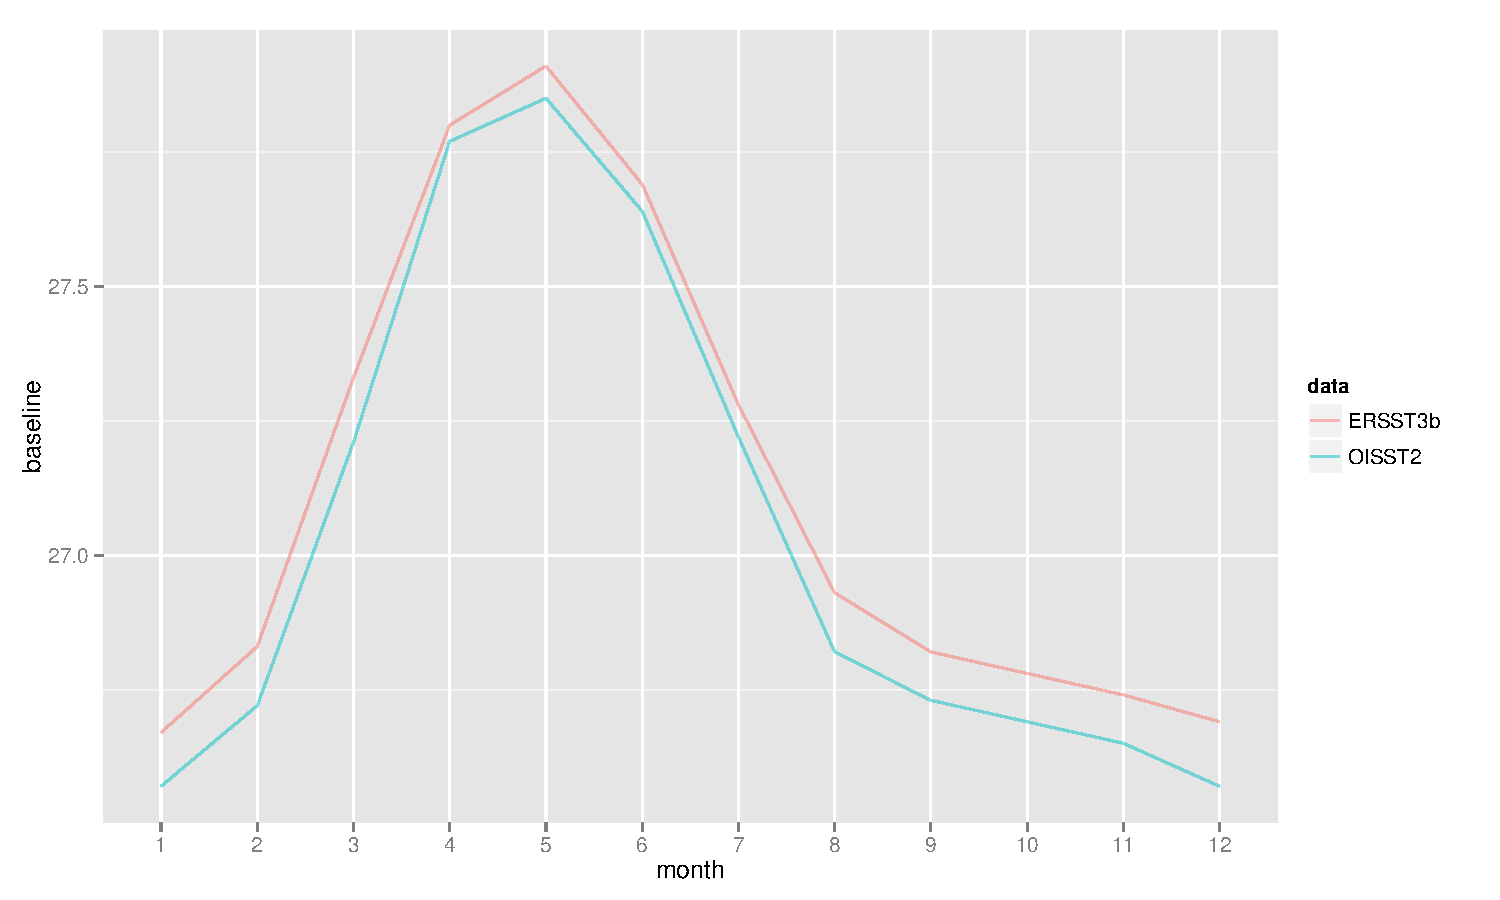
\includegraphics[width=\linewidth]{Pricingfigs/CompareOISSTandERRSTbaselines}
  \caption{Comparing OISST and ERSST monthly baselines}
   \label{fig:baeslinesOIER}
\end{figure*}

The key factor distinguishing ERSST from OISST is the use of in-situ or satellite data. ERSST exclusively uses in-situ measurement, primarily that consists of temperature readings taken by a network of buoys throughout the Pacific (which are now communicated via sattelite) \cite{smith2004improved}\cite{smith2003extended}\cite{smith2008improvements}. Monthly anomalies in the ERSST version 3b index are measured relative to a 1971-2000 base period with a resolution of two degrees across the four ENSO regions\cite{xue2003interdecadal}. While the primary index record that NOAA posts to its websites goes back to 1950, monthly ERSST data are available from 1854 on.

OISST, currently at version 2, combines in situ SST measurements, daytime and nighttime satellite data readings, and data from sea ice cover simulations. The satellite-measured data, whose collection began in the early 1980s, is adjusted statistically for natural sources of bias, like cloud cover and atmospheric water vapor\cite{reynolds2002improved} \cite{reynolds1994improved} \cite{reynolds1993improved} \cite{reynolds1988real}. 

Finance professionals require reliability, simplicity, and a long track record of their settlement indexes. Neither ERSST nor OISST has a clear advantage along all three axes. OISST is more diversified in its data sources. That may make the index more reliable than ERSST, which requires buoys subject to physical damage. At times, NMS must extrapolate data for buoys that are offline and that extrapolation introduces subjectivity into ERSST.

However, OISST will likely be considered more complicated that ERSST. It combines data from multiple sources in a procedure that requires some advanced climate knowledge to parse. The statistical treatment of OISST is important to the final index. Satellite measurements of Pacific SSTs have to date shown a \emph{cold bias}, suggesting temperatures that were too cold relative to in situ measurement by a factor of .01 deg C. (For that reason NOAA discontinued the issuance of ERSST version 3, which did attempt to add some satellite measured data.) ERSST relies by contrast on data procedures that are relatively simple for non-experts to grasp - buoys take temperature readings at regular intervals and relay that information via satellite.

The reason that we believe that ERSST is ultimately a better index for financial contract settlement is its age. ERSST simply offers a longer time series for actuarial analysis. Using ERSST, gives practitioners almost thirty-five additional historical data points for any given month. Those extra data points provide everyone involved with a great deal more confidence in their pricing models. 

\subsection{Choosing a region}
Ni\~no 1.2 is the best predictor of catastrophic flooding in Peru and Ecuador consequently it was the basis for the existing El Ni\~no's insurance \cite{khalil2007nino}. However, NMS generally mark ENSO anomalies using the Ni\~no 3.4 region, which stretches across the central Pacific \cite{barnston1997documentation}. Both regions, Ni\~no 1.2 and the Ni\~no 3.4, have a very high correlation during extreme anomalies. But Ni\~no 3.4 is generally considered a better proxy for the worldwide teleconnections associated with ENSO. In particular, it does a better job capturing ENSO anomalies with different geographic signatures. During the 1972/1973 El Ni\~no, for example, most of the sea-surface temperature warming occurred in the central Pacific, closer to Ni\~no 3.4. El Ni\~no events focused on the Central Pacific are also called \emph{Modoki} Ni\~nos and can have large global impacts \cite{ashok2007Nino}.

\subsection{Choosing a format}
After selecting a settlement index, market innovators must also choose the format in which settlement numbers will be presented to traders. In the case of ENSO, that choice centers on the question of whether to use: 
\begin{itemize}
\item Anomalies (degree Celsius departures from monthly averages) or absolute degrees Celsius; and,
\item Simple monthly values or moving averages, with for example, a three month window.
\end{itemize}

Regarding anomalies, its not immediately clear which format is better for financial contracts. The work here is presented in terms of absolute values to mirror the format of the existing El Ni\~no insurance. By contrast, most major meteorological organizations define those events in terms of persistent monthly anomalies. Indeed, many forecasts of SSTs (like those from the ABM and IRI) are only provided in terms of anomalies. So, early traders may feel more comfortable thinking in terms of anomalies.

The primary disadvantage of anomalies is that they have been, and will continue to be, subject to revision as underlying SSTs drift over time. There appears to be a link between climate change and higher Pacific SSTs and some scientist have outlined plausible scenarios in which we enter into a permanent Ni\~no state INCLUDE CITATION. To the extent that such trends continue, the index may revise its baseline and the interpretation of anomalies may become less clear. 

Changing baselines are not a serious problem in similar markets. Many weather derivative use annually revised baselines. However, absolute measurements will directly incorporate any underlying shifts in the index, allowing, for example, traders to simply express theories about the long-term trends in the index. Those theories and, by proxy, the market's judgment of long-term climate change might be obscured in an anomaly-based contract.

The choice between using individual monthly values and rolling windows is more straight-forward. While rolling averaged indexes are actually what NOAA uses to define ENSO and what GlobalAgRisk used for it's insurance contract, monthly positions allow for greater flexibility. If there were traded markets on monthly values, it would be trivial for traders to combine positions and create a position that mirrors a single contract settled on a three-month rolling average. Combining rolling average positions to produce individual monthly positions is more difficult. Consequently, we have focused on monthly values here.

\section{Developing a prototypical contract}
Now that we have a target index, we can begin the process of pricing that contract. That process involves:
\begin{itemize}
 \item Choosing a pricing function to convert index values into financial obligations;
 \item Running historical values through that pricing function, and 
 \item Fitting a distribution to historical values to generate prices that reflect the underlying statistical process of ENSO. 
\end{itemize}
Based on the recommendation of Dr. Andrew Watkins of the Australian Bureau of Meteorology (ABM) we have chosen to use October as our example month, since October values of Ni\~no 3.4 tend to be critical in identifying El Ni\~no/La Ni\~na worldwide. 

\subsection{Pricing function}
Extreme El Ni\~no/La Ni\~na, will drive early hedging. Consequently, we have focused on financial contracts that are well-suited to representing extreme risk such as options. Options have \emph{triggers}, index values that mark the start and end of contingent liabilities. We have selected triggers of one and three standard deviations away from the monthly mean.  Payments on our example options begin at one standard deviation above (for a \emph{call} option covering El Ni\~no) or below (for a \emph{put} option covering La Ni\~na) the monthly average. Payments reach one hundred percent of the notional value (or sum insured) at three standard deviations above or below the monthly average for El Ni\~no/call and La Ni\~na/put contracts respectively. Figure \ref{fig:optionParamsByMonth} shows the average monthly value for Ni\~no 3.4 in black. The red and blue bands show the index values for each month that would trigger a payment on calls and puts respectively.

\begin{figure*}[!htbp]
  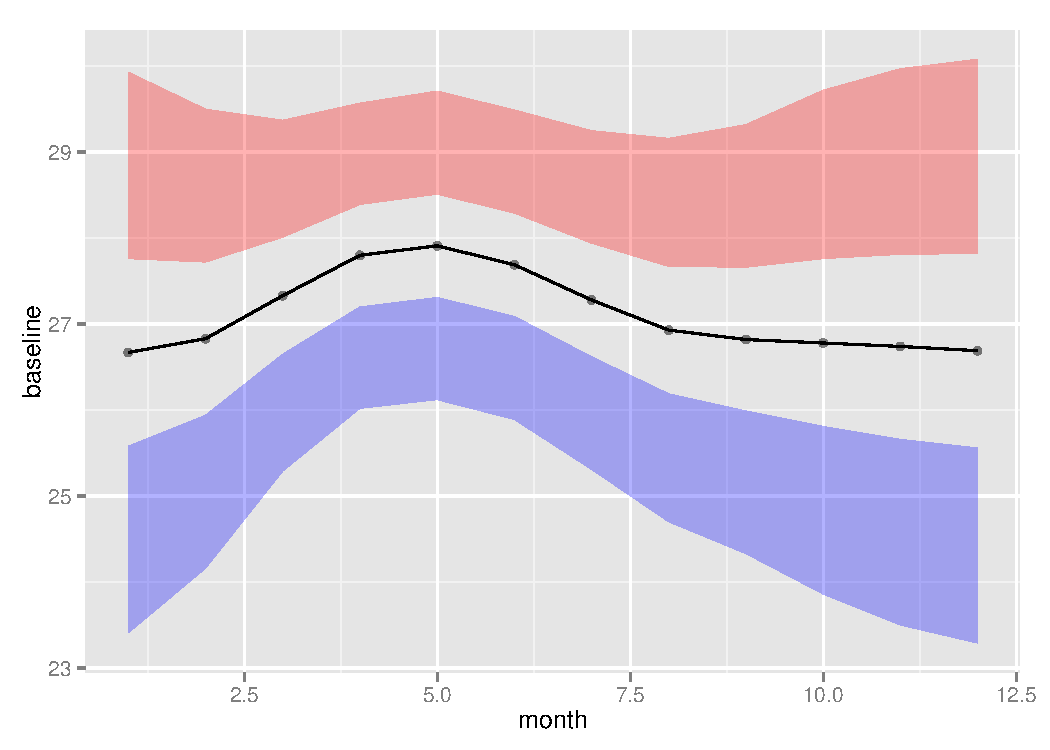
\includegraphics[width=\linewidth]{Pricingfigs/optionParamsByMonth}
  \caption{Index values for El Ni\~no (red) and La Ni\~na (blue) events between one and three standard deviations away from monthly average}
   \label{fig:optionParamsByMonth}
\end{figure*}

Within those ranges, we use linear pricing such that an index value halfway across the red band in figure \ref{fig:optionParamsByMonth} (i.e. halfway between the the trigger and max payout point) would obligate a payout that is half of the sum insured on a call/El Ni\~no contract. The full linear function for October El Ni\~no is shown in figure \ref{fig:payouyt10callex}. 

\begin{figure*}[!htbp]
  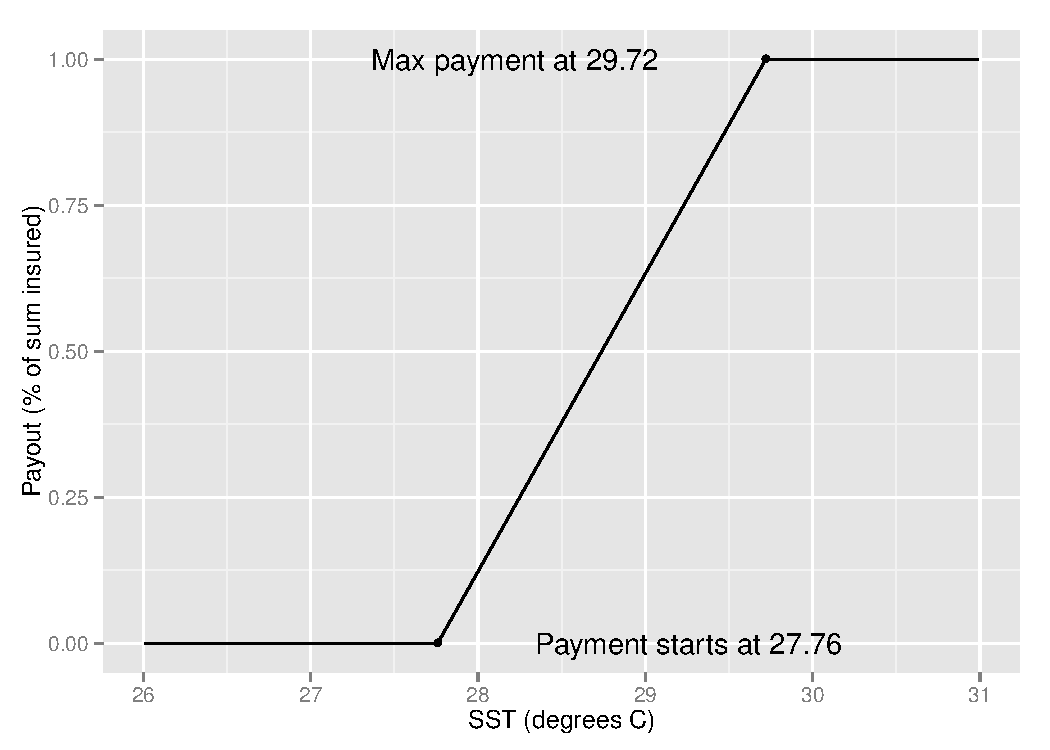
\includegraphics[width=\linewidth]{Pricingfigs/payoutExamplemonth10contractType1}
  \caption{Payout function for call option (equivalent to El Ni\~no coverage) on October SST for Ni\~no 3.4 ERSST.3b trigged by index values between one and three standard deviations above the monthly baseline.}
   \label{fig:payouyt10callex}
\end{figure*}

As an example, suppose that a Peruvian bank bought USD $100$ of coverage (we will deal with the price of that coverage below) against October El Ni\~no. If actual October SST was halfway across the red band, or $28.74^{\circ}\mathrm{C}$, I would receive USD $50$.

In practice, GlobalAgRisk found that hedgers (and speculators) prefer a payout function that offers a minimum payout in the event that the index reaches just above the trigger. For example, an index value that just barely crosses into the red in \ref{fig:optionParamsByMonth} might trigger a payout of $5$ percent on an El Ni\~no/call contract, rather than the tiny payout suggested the kind of linear function in figure \ref{fig:payouyt10callex}.

% Some potential clients also expressed interest in a more customized payout function consisting of steps usually shaped around historical events e.g. a 25 percent payout for the 1972/1973 magnitude event and a 75 percent for a 1997/1998 magnitude event.

\subsection{Distribution}
With a pricing function in hand, we can provide basic prices for El Ni\~no and La Ni\~na risk protection, using both historical data (pricing based on historical data alone is called \emph{burn analysis} in the world of insurance) and using random samples from distributions fit to that historical data. The process for fitting distributions to weather and climate data and generating insurance and derivatives prices from those distributions has been covered elsewhere INCLUDE REFERENCE TO JEWSON. Here we cover them only to provide reader with a sense of the uncertainty facing sellers of this risk, even prior to the introduction of forecasting which may result in asymmetric information. 

The prices in figure \ref{fig:optionPricesWithVariousDistMonth} are unconditional on forecasts meaning that they are equivalent to actuarially-fair insurance prices that could be offered prior to an insurance sales closing date. They are denominated in USD of premium per USD 100 of nominal coverage. The figure includes burn prices, prices from a sample taken from a non-parametric kernel density smoother fit to historical data, as well as prices based on various distributional fits. 

\begin{figure*}[!htbp]
  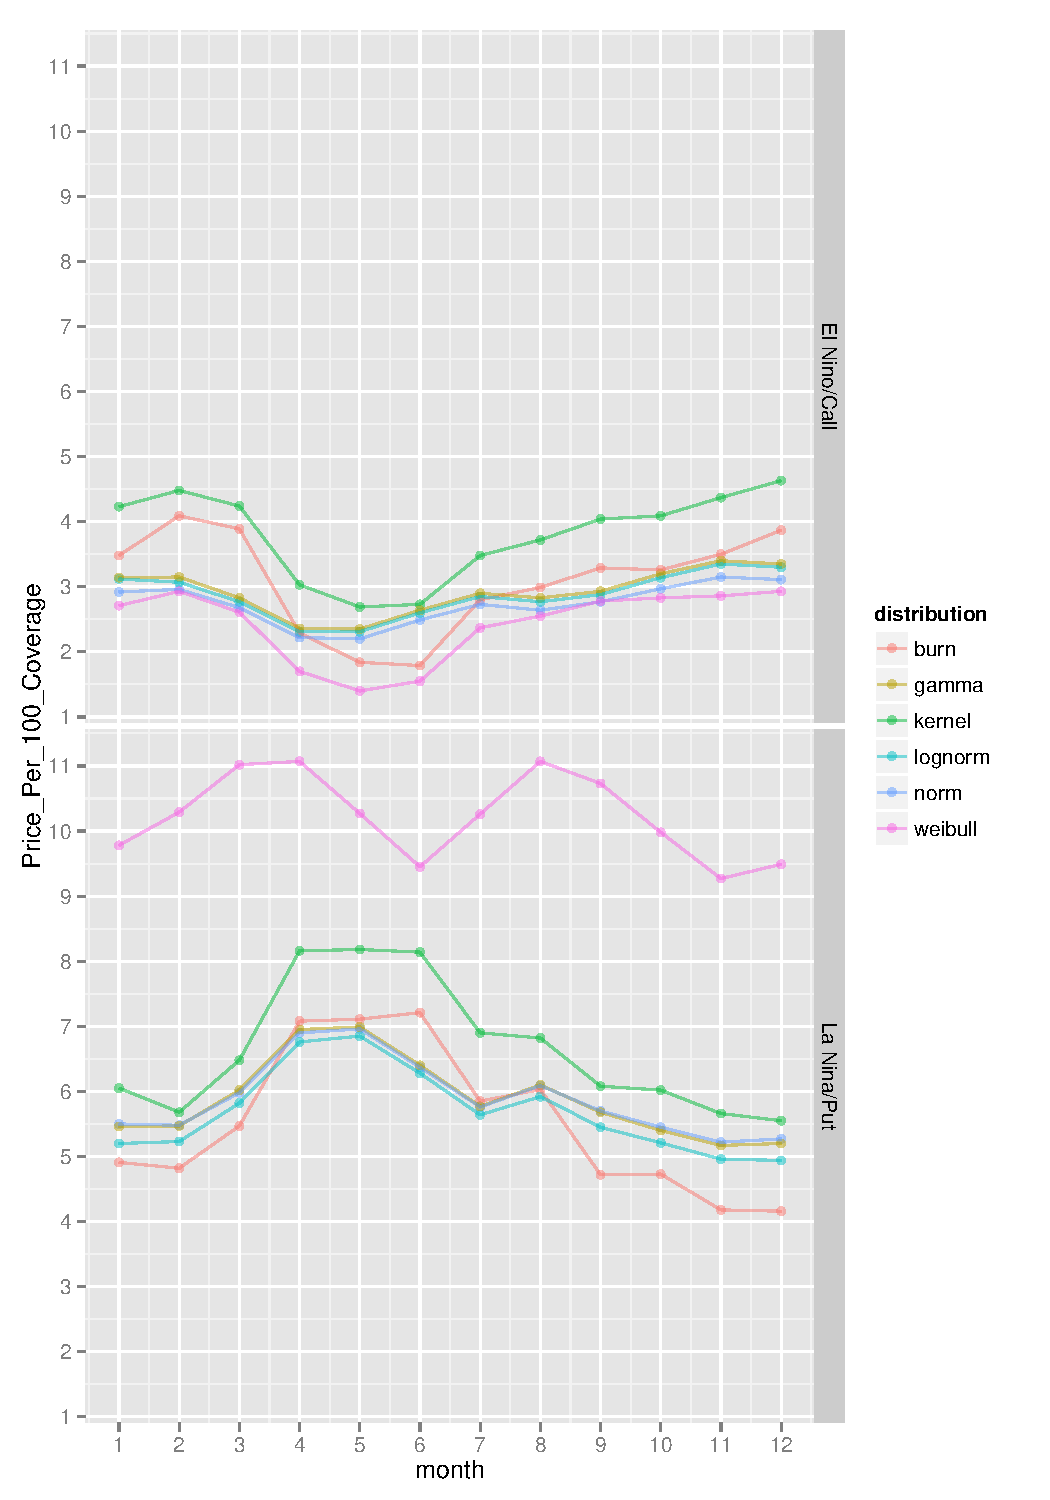
\includegraphics[width=\linewidth]{Pricingfigs/optionPricesWithVariousDistMonth}
  \caption{Expected price for options on Ni\~no 3.4 by month, based on simulations from various distributions}
   \label{fig:optionPricesWithVariousDistMonth}
\end{figure*}

The prices in figure \ref{fig:optionPricesWithVariousDistMonth} may appear, with one prominent exception\footnote{The prices from the Weibull samples are clearly distinct from the rest of the group - almost doubling the price of La Ni\~na coverage relative to the rest of the group. That is understandable given the distribution's heavy left tail. There is no indication that the process generating ENSO SST has a heavy left tail, so the distribution may not be appropriate here.}, close to one another. However, they remain far enough apart that hedgers would certainly notice a difference between the prices offered by speculators insisting on the most conservative pricing assumptions an those of speculators willing to offer coverage at prices matching some weighted model average. On the El Ni\~no side, the highest and lowest prices are generally within 125 basis points (1.25 percent) of one another in any given month. On the La Ni\~na side, that spread is slightly larger at roughly 150 basis point, but only between April and June. 

As we will discuss later, a common heuristic for non-traditional risk premiums in catastrophe bond markets (those risks which are rarely managed in catastrophe bond markets and thus are valued for their diversification benefits) is that speculators demand a premium of 400 basis points above expected loss. Using that benchmark, an October call covering El Ni\~no events between one and three standard deviations from the monthly baseline priced using the normal distribution might cost roughly 675 basis points. The same call priced using a kernel density smoother might cost 800 basis points, almost 20 percent higher than a hedge priced using the normal distribution. 

The implied price difference illustrates two important points for climate scientists looking to encourage the development of markets for protection against the risks they study. First, distributional assumptions have important economic consequences for risk markets settling on direct climate indexes, even before considering the added complication of forecasts. In the case of ENSO, there is past climate literature which uses a normal distribution to model ENSO. As we discuss in the next section, we follow that precedence here while allowing room for key modeling parameters to shift across a large search space. However, further research on the appropriate distributions for pricing climate risks will expedite the formation of stable, active risk markets.

The second important point to take away from figure \ref{fig:optionPricesWithVariousDistMonth} is that the launch of ENSO and similar direct climate markets require a simple and transparent means of dealing with modeling uncertainty. In the following section we present such a approach to pricing climate risk with many sources of uncertainty.

\section{Pricing ENSO risk contingent on available forecasts: quantifying forecast error to encourage trading}
As discussed, extreme El Ni\~no/La Ni\~na events emerge over time, with forecasts giving us ever more reliable information in the months leading up to a given event changing the beliefs of ENSO watchers. We have discussed how ENSO risk prices that reflected those changing beliefs  could improve social welfare. However, the trading activity that would provide those prices may be undermined in the absence of pricing tools that offer a benchmark for ENSO risk traders, mitigating the risk of trading in the presence of asymmetric information. Reliable and clear public information on prices narrows the range within which relatively naive traders can make mistakes about pricing. Some highly specialize traders may still retain a consistent edge over traders pricing exclusively off of this public baseline, but their profit margins will diminish as public information improves.

This section provides such a benchmark. We present statistical simulations of monthly Ni\~no 3.4 sea surface temperatures conditioned on average forecasts released by Colombia University's International Research Institute for Climate and Society (IRI). We use those simulations to update the prices of risk management contracts as new forecast information becomes available.

\subsection{Forecasts of ENSO SSTs}
Before discussing the statistical treatment of forecasts, it is worth quickly reviewing the ENSO SST forecasts provided by IRI because those forecasts are offered in a format that is not directly comparable to the format we believe is most appropriate for traded Ni\~no risk protection. 

Every month since mid-2002, IRI has collected forecasts issued by major centers of climatological research. Figure \ref{fig:forecastExamples} shows IRI the forecasts as of March 2013.

\begin{figure}
  \begin{center}
  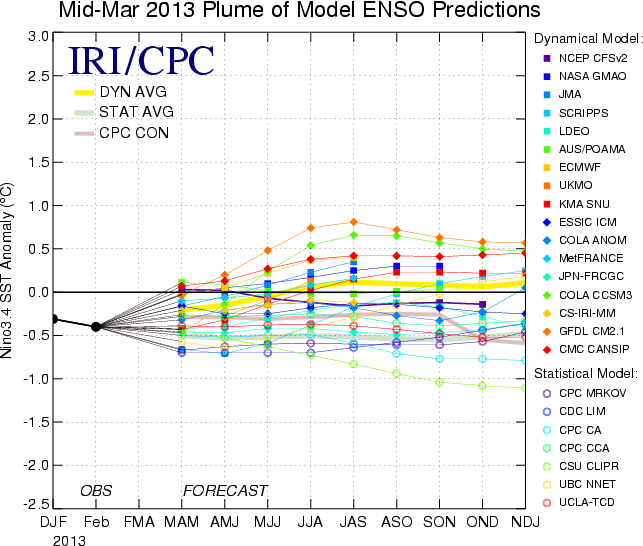
\includegraphics[width=.5\linewidth]{Pricingfigs/SST_table_march_ex}
  \caption{Example of IRI's collected forecasts - March 2013}
   \label{fig:forecastExamples}
   \end{center}
\end{figure}

IRI provides Ni\~no 3.4 anomaly SST forecasts over three month rolling windows. As discussed previously, monthly SSTs are likely better suited to risk trading. To provide an index of IRI  forecasts that is directly comparable to the monthly SSTs that we wish to price, we have averaged all the available IRI forecasts that cover a given month. For an example of how we made this simplification, imagine that it is March and a hedger is interested in predicting October Ni\~no 3.4 SST. In figure \ref{fig:forecastExamples}, there are three forecasts that contain information relevant to October SSTs - \emph{ASO}, \emph{SON}, and \emph{OND}. In that case our forecast index is the average of those three numbers. 

IRI issues forecasts between 2 and 10 months prior to any given target month. For example, October SST forecasts begin in December and end in September. 

\subsection{Linking forecasts to outcomes ENSO SSTs}
We generate stochastic catalogues of ENSO outcomes conditional on the IRI average forecasts discussed above using the Bayesian regression shown in equation \ref{eqn:conditionalEstEqn}. This a simplified version of a procedure that climate scientists and statisticians have recently used to merge ENSO forecasts\cite{luo2007bayesian}\cite{coelho2004forecast}. Since we want pricing for every month, from the vantage-point of every preceding month with IRI forecasts, we run a total of $108$ separate regressions. 

Note first that we do not know the predictive power of IRI average forecasts a priori. The parameter $\sigma_{y_{month,forecast month}}^2$ accounts for that forecasting uncertainty. It will be large where IRI average forecasts have shown low historical predictive power. Note also that this Bayesian regression will not be biased by non-stationarity. The underlying parameters are not assumed to be stationary, since they are realizations of an unknown distribution.

\begin{equation}
\begin{array}{lcl}
\mbox{Monthly Ni\~no 3.4 ERSST.3b anomalies}_{month,year} & \sim & \mathcal{N}( \hat{y}_{month,forecast month,year}, \sigma_{y_{month,forecast month}}^2 )\\
\hat{y}_{month,forecast month,year} & = & a_{month,forecast month} \\
&& + b_{month,forecast month}*\\
&& \mbox{average of IRI average forecasts}_{month,forecast month}\\
\end{array}
\label{eqn:conditionalEstEqn}
\end{equation}

The prior probabilities placed on model parameters are shown in equation set \ref{eqn:priorsconditionalEstEqn}. There are weakly informative priors on $b$ and $\sigma_{y}$, allowing them to move easily across a wide range of possible values in response to the data. $a$ by contrast has a strongly informative prior based on historical data. This means that if $b$, the parameter indicating the predictive power of IRI's average forecasts, is at or near zero, then the resulting simulations from the posterior distribution will simply reflect long term trends in monthly SSTs.

\begin{equation}
\begin{array}{lcl}
a_{month,forecast month}  & \sim & \mathcal{N}(\mbox{mean anomalies}_{month}, \mbox{st dev anomalies}_{month}) \\
b_{month,forecast month}  & \sim & \mathcal{N}(0, 100) \\
\sigma_{y_{month,forecast month}}^2 & \sim  &\mbox{Inv gamma}(0.001, 0.001) \\
\end{array}
\label{eqn:priorsconditionalEstEqn}
\end{equation}

\subsubsection{Dynamic pricing based on model results}
The table below contains regression results for October SSTs, predicted between the preceding December and August. The regressions were all estimated using the Bayesian estimation program STAN with four parallel Markov Chain Monte Carlo (MCMC) chains, each with 100,000 iterations, 50,000 of which were discarded as a warm-up\cite{stan2013}. The convergence statistic, $\hat{R}$, on all parameters was close to 1, indicating that the parallel MCMC chains showed similar results by the end of the simulation.

\begin{table*}[ht]
\centering
\footnotesize
\begin{tabular}{rrrrrrrrrr}
\hline
\multicolumn{10}{c}{August forecast average covering October Ni\~no 3.4 SST anomalies}\\

  \hline
 & mean & sd & $2.5^{\mbox{th}}$ q & $25^{\mbox{th}}$ q & $50^{\mbox{th}}$ q & $75^{\mbox{th}}$ q & $97.5^{\mbox{th}}$ q & n\_eff & Rhat \\ 
  \hline
$\alpha$ & -0.10 & 0.10 & -0.40 & -0.20 & -0.10 & -0.10 & 0.10 & 91045 &   1 \\ 
  $\beta$ & 1.10 & 0.20 & 0.80 & 1.00 & 1.10 & 1.20 & 1.50 & 88920 &   1 \\ 
  $\sigma^{2}_{y}$ & 0.10 & 0.10 & 0.10 & 0.10 & 0.10 & 0.20 & 0.40 & 56829 &   1 \\ 
   \hline
\hline
\multicolumn{10}{c}{July forecast average covering October Ni\~no 3.4 SST anomalies}\\
  \hline
$\alpha$ & -0.10 & 0.20 & -0.50 & -0.20 & -0.10 & 0.00 & 0.20 & 92218 &   1 \\ 
  $\beta$ & 1.20 & 0.30 & 0.60 & 1.00 & 1.20 & 1.30 & 1.70 & 93712 &   1 \\ 
  $\sigma^{2}_{y}$ & 0.30 & 0.20 & 0.10 & 0.20 & 0.30 & 0.40 & 0.90 & 54297 &   1 \\ 
   \hline
\hline
\multicolumn{10}{c}{June forecast average covering October Ni\~no 3.4 SST anomalies}\\
  \hline
$\alpha$ & -0.10 & 0.20 & -0.40 & -0.20 & -0.10 & 0.00 & 0.30 & 95908 &   1 \\ 
  $\beta$ & 1.40 & 0.30 & 0.70 & 1.20 & 1.40 & 1.60 & 2.10 & 91107 &   1 \\ 
  $\sigma^{2}_{y}$ & 0.30 & 0.20 & 0.10 & 0.20 & 0.30 & 0.40 & 0.90 & 55596 &   1 \\ 
   \hline
\hline
\multicolumn{10}{c}{May forecast average covering October Ni\~no 3.4 SST anomalies}\\
  \hline
$\alpha$ & -0.10 & 0.20 & -0.50 & -0.20 & -0.10 & 0.10 & 0.40 & 92919 &   1 \\ 
  $\beta$ & 1.50 & 0.60 & 0.40 & 1.20 & 1.50 & 1.90 & 2.60 & 90255 &   1 \\ 
  $\sigma^{2}_{y}$ & 0.50 & 0.30 & 0.20 & 0.30 & 0.50 & 0.60 & 1.40 & 59205 &   1 \\ 
   \hline
\hline
\multicolumn{10}{c}{April forecast average covering October Ni\~no 3.4 SST anomalies}\\
  \hline
$\alpha$ & -0.10 & 0.20 & -0.50 & -0.30 & -0.10 & 0.00 & 0.30 & 88326 &   1 \\ 
  $\beta$ & 1.90 & 0.60 & 0.70 & 1.50 & 1.90 & 2.30 & 3.00 & 83902 &   1 \\ 
  $\sigma^{2}_{y}$ & 0.40 & 0.30 & 0.20 & 0.30 & 0.40 & 0.50 & 1.10 & 57674 &   1 \\ 
   \hline
\hline
\multicolumn{10}{c}{March forecast average covering October Ni\~no 3.4 SST anomalies}\\
  \hline
$\alpha$ & 0.00 & 0.20 & -0.50 & -0.10 & 0.00 & 0.20 & 0.50 & 101040 &   1 \\ 
  $\beta$ & 1.80 & 0.90 & 0.00 & 1.20 & 1.80 & 2.30 & 3.50 & 96782 &   1 \\ 
  $\sigma^{2}_{y}$ & 0.70 & 0.50 & 0.30 & 0.50 & 0.60 & 0.90 & 1.90 & 59539 &   1 \\ 
   \hline
\hline
\multicolumn{10}{c}{February forecast average covering October Ni\~no 3.4 SST anomalies}\\
  \hline
$\alpha$ & -0.10 & 0.30 & -0.70 & -0.30 & -0.10 & 0.10 & 0.60 & 98192 &   1 \\ 
  $\beta$ & 0.80 & 1.30 & -1.80 & 0.00 & 0.80 & 1.60 & 3.40 & 88684 &   1 \\ 
  $\sigma^{2}_{y}$ & 1.10 & 0.80 & 0.40 & 0.60 & 0.90 & 1.30 & 3.20 & 54912 &   1 \\ 
   \hline
\hline
\multicolumn{10}{c}{January forecast average covering October Ni\~no 3.4 SST anomalies}\\
  \hline
$\alpha$ & 0.00 & 0.30 & -0.60 & -0.20 & 0.00 & 0.20 & 0.60 & 99518 &   1 \\ 
  $\beta$ & 1.00 & 1.60 & -2.30 & 0.00 & 1.00 & 2.00 & 4.20 & 92225 &   1 \\ 
  $\sigma^{2}_{y}$ & 1.00 & 0.70 & 0.40 & 0.60 & 0.80 & 1.20 & 2.80 & 55715 &   1 \\ 
   \hline
\hline
\multicolumn{10}{c}{December forecast average covering October Ni\~no 3.4 SST anomalies}\\
  \hline
$\alpha$ & 0.00 & 0.30 & -0.60 & -0.20 & 0.00 & 0.30 & 0.70 & 80946 &   1 \\ 
  $\beta$ & -0.30 & 1.90 & -4.00 & -1.40 & -0.30 & 0.90 & 3.50 & 76663 &   1 \\ 
  $\sigma^{2}_{y}$ & 1.10 & 0.70 & 0.40 & 0.60 & 0.90 & 1.30 & 2.90 & 56323 &   1 \\ 
   \hline
\end{tabular}
\caption[Bayesian regression linking October Ni\~no 3.4 SST anomalies to average of relevant IRI ensemble forecasts]{Bayesian regression linking October Ni\~no 3.4 SST anomalies to average of relevant IRI ensemble forecasts} 
\end{table*}


Looking at the 2.5th and 97.5th percentile of the distributions for $b$, its clear that the forecasts become more valuable predictors as the year goes on. Going from December to August, the 95 percent probability interval for the forecast parameter, $b$ steadily tightens to a range including 1. This suggest that the correlation between forecasts and eventual SSTs increases throughout the predictive window. As the explanatory value of $b$ increases, $a$ decreases. $a$'s 95 percent probability tightens around 0 after March indicating that there are no consistent patterns of IRI forecasts being too high or too low relative to observed SSTs after March.

Using the posterior draws of parameter values from these 108 regressions, we simulated SSTs predicted by each possible forecast value between -2 and 2 (forecasts are rounded to one decimal). For example, we took 50,000 posterior draws of $a$, $b$, and $\sigma_{y}^2$ from the regression corresponding to October SSTs predicted by April forecasts. Each of those 50,000 vectors of three parameters were used to randomly generate one October SST based on an average April forecast of mild El Ni\~no conditions in the coming October (a forecast value of 0.5). That gave a stochastic catalog of 50,000 October SSTs conditioned on a forecast of 0.5 made in April. We repeated that procedure to produce conditional distributions for SSTs for each month of the year, predicted by a wide range of forecast values, from all possible forecast months. 

The empirical cumulative distribution functions (ECDFs) of those posterior simulations, converted back into absolute SSTs, are shown in figures \ref{fig:conditionalCDFs04to06}, \ref{fig:conditionalCDFs07to09}, \ref{fig:conditionalCDFs10to12}, and \ref{fig:conditionalCDFs01to03}. \footnote{We have also touched on why the choice between anomalies and absolute SSTs is of lower importance than some of the other choices facing the launch of traded ENSO markets. Our statistical routines linking forecasts to outcomes are in terms of anomalies. However, financial professionals unfamiliar with ENSO SST indexes may benefit from seeing the absolute temperates because they show the natural fluctuations in Pacific SSTs throughout the year which have been taken out of anomaly figures. In recognition of that fact, the conditional cumulative distribution functions below are in terms of absolute degrees.}

\begin{figure*}[!htbp]
  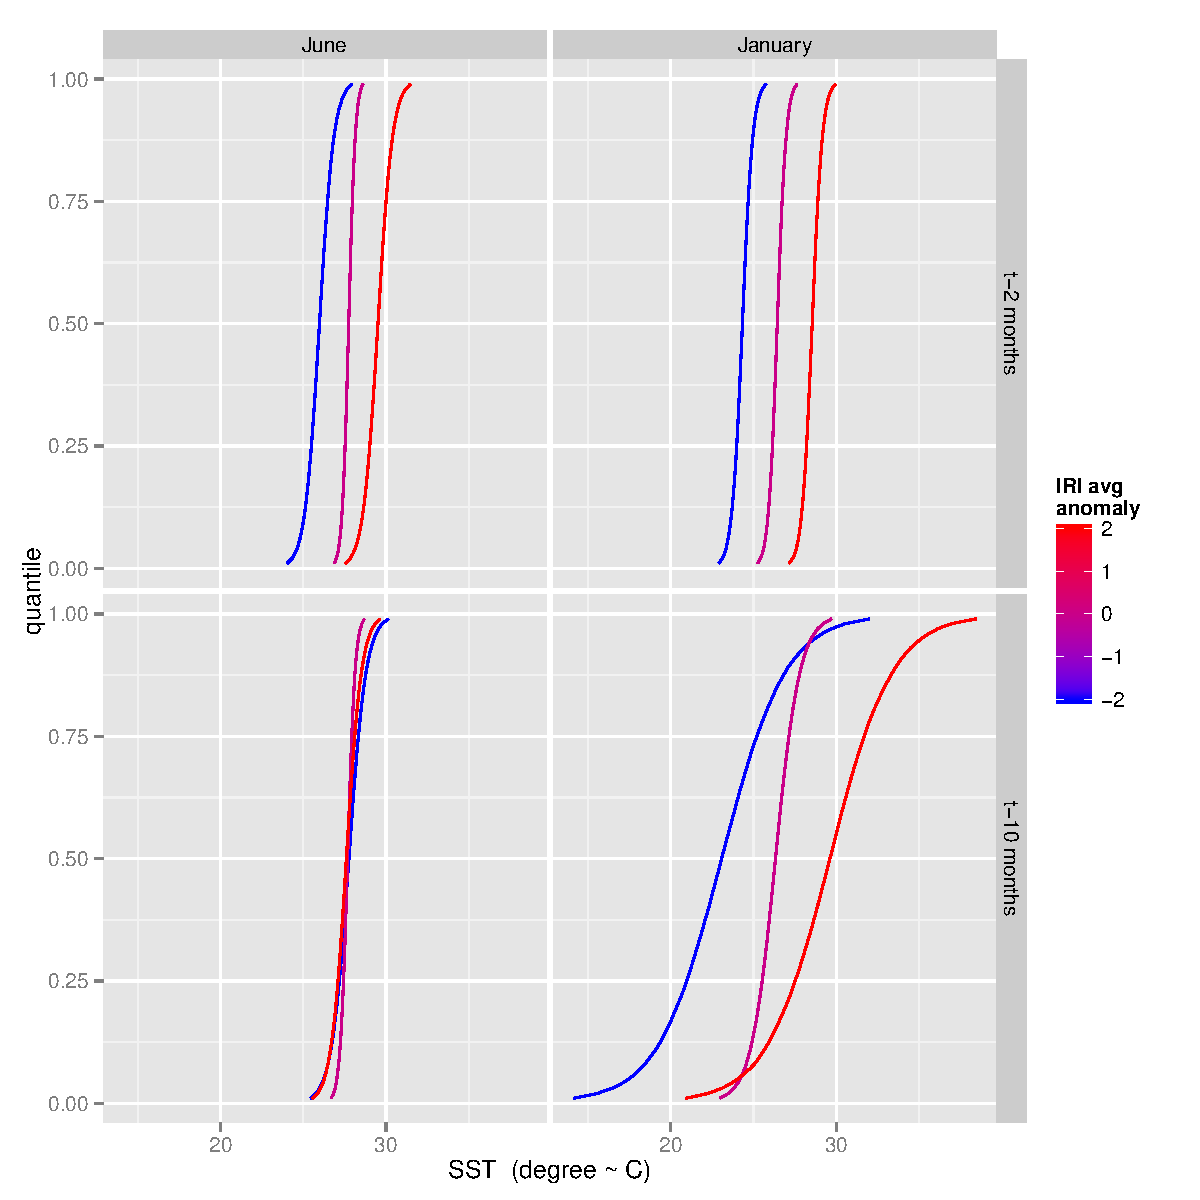
\includegraphics[width=\linewidth]{Pricingfigs/conditionalCDFsIllustrativeExamplesTradConfigSimple}
  \caption{Empirical cumulative distribution functions for June and January Ni\~no 3.4 SST conditioned on average IRI ensemble forecasts available for various months. Only the ECDFs for the nearest and furthest month predictions provided by IRI and only predictions of large El Ni\~no (+2), La Ni\~na (-2), or neutral conditions (0) are shown. ECDFs are of draws from the posterior predictive distribution of the model specified in equation \ref{eqn:conditionalEstEqn}.}
   \label{fig:conditionalCDFsIllustrativeExamplesTradConfigSimple}
\end{figure*}

Figure \ref{fig:conditionalCDFsIllustrativeExamplesTradConfigSimple} presents a highly simplified example of these ECDFs. It has just two target months (June and January), two windows from which predictions of SSTs in those target month were made (two and ten months prior to the target month) and three prediction values (a +2 anomaly suggesting strong El Ni\~no, indicated by the deepest red line, a -2 anomaly suggesting strong La Ni\~na, indicated by the deepest blue line, and no anomaly suggesting neutral conditions, indicated by the purple line). The highest simulated SSTs conditioned on a given forecast at then upper right-hand end of each line, with the simulation result value on the x-axis and the quantile of that result on the y-axis.

The pattern of these ECDFs tell a great deal about the predictive power of IRI average forecasts and the underlying process of SSTs in a given month. Note first that June simply is not a month with highly variable SSTs. The purple line indicating the ECDF conditioned on neutral forecasts is almost vertical, both when those forecasts are made in April and in  August of the preceding year. January SSTs show greater underlying variability, with their ECDFs stretching further along the x-axis.

The longest dated forecasts (t-10 months) are not reliable for June but show some value for January. This is shown by the overlap of the various ECDFs. In June, they are stacked on top of one another, showing that conditioning on forecasts produces roughly equivalent distributions of outcomes. By contrast, extreme forecasts of El Ni\~no or La Ni\~na were associated with January SSTs that were distributionally distinct from one another (there is little overlap between the lower tail of the red line and the upper tail of the blue line) the with high confidence, even for forecasts made in March. However, while a March forecast of El Ni\~no conditions in January meant that we were unlikely to see extreme La Ni\~na conditions, it did not rule out the range of outcomes associated with neutral forecasts.

By the time that we are only two months away from our target months however, extreme high and low forecasts are associated with a range of outcomes that are distinct both from one another and from neutral forecasts. This shows how the informational value of forecasts increases as the forecast horizon gets shorter.

In figure \ref{fig:conditionalCDFsIllustrativeExamplesTradConfigFull} the full complement of forecasts is shown for the same targets and forecast horizons. Boxes where the red lines are consistently above the blue lines indicate high informational value for forecasts, with a clear distinction between outcomes associated with high and low forecasts.

\begin{figure*}[!htbp]
  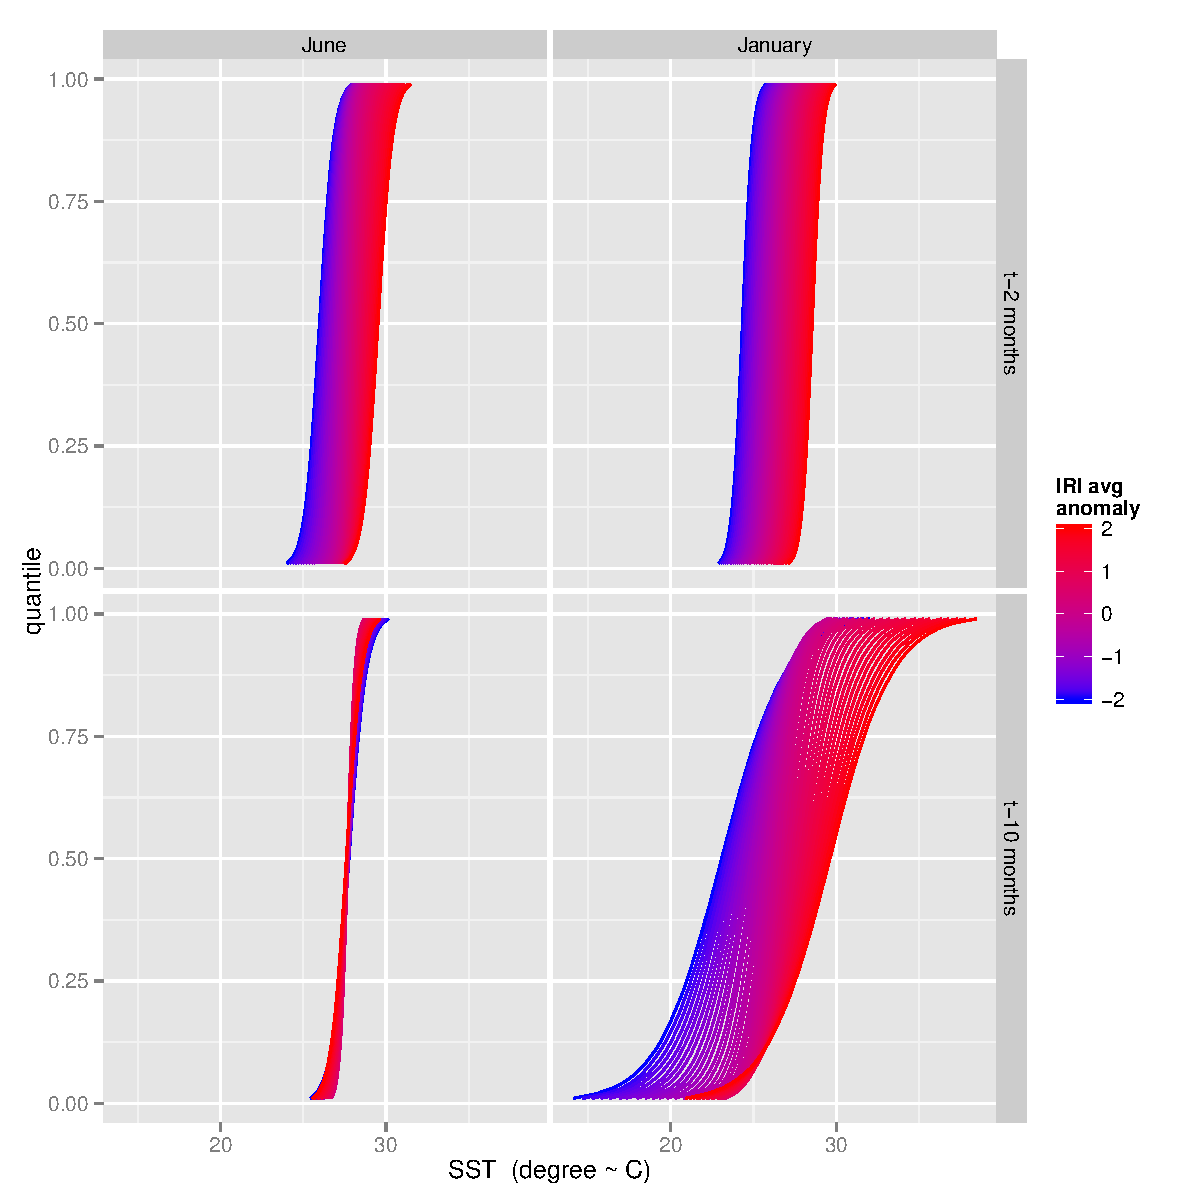
\includegraphics[width=\linewidth]{Pricingfigs/conditionalCDFsIllustrativeExamplesTradConfigFull}
  \caption{Empirical cumulative distribution functions for June and January Ni\~no 3.4 SST conditioned on average IRI ensemble forecasts available for various months. Only the ECDFs for the nearest and furthest month predictions provided by IRI are shown. ECDFs are of draws from the posterior predictive distribution of the model specified in equation \ref{eqn:conditionalEstEqn}.}
   \label{fig:conditionalCDFsIllustrativeExamplesTradConfigFull}
\end{figure*}

 % fig:conditionalCDFsJantoJune
 % fig:conditionalCDFsJultoDec

% \ref{fig:conditionalCDFsJantoJune} and \ref{fig:conditionalCDFsJultoDec}

 % \ref{fig:conditionalCDFs04to06}, \ref{fig:conditionalCDFs07to09}, \ref{fig:conditionalCDFs10to12}, and  \ref{fig:conditionalCDFs01to03}

With that simplified example in mind you can interpret patterns in the full simulation results shown in figures \ref{fig:conditionalCDFs04to06}, \ref{fig:conditionalCDFs07to09}, \ref{fig:conditionalCDFs10to12}, and \ref{fig:conditionalCDFs01to03}. As in the simplified example, the blue and red lines are tightly bound ten months prior to any given target month and in many cases the blue lines reach further right than the red. This indicates that forecasts had little or no predictive power. Warm forecasts were as closely associated with eventual warm conditions as cold forecasts, and visa versa. 

By contrast, two months away from a target month (the upper row of figures \ref{fig:conditionalCDFs04to06}, \ref{fig:conditionalCDFs07to09}, \ref{fig:conditionalCDFs10to12}, and \ref{fig:conditionalCDFs01to03}), forecasts are meaningful. Blue lines sit below red lines. So a warm forecast shifts the distribution of eventual SSTs warmer and visa versa.

\begin{figure}[!htbp]
\begin{center}
  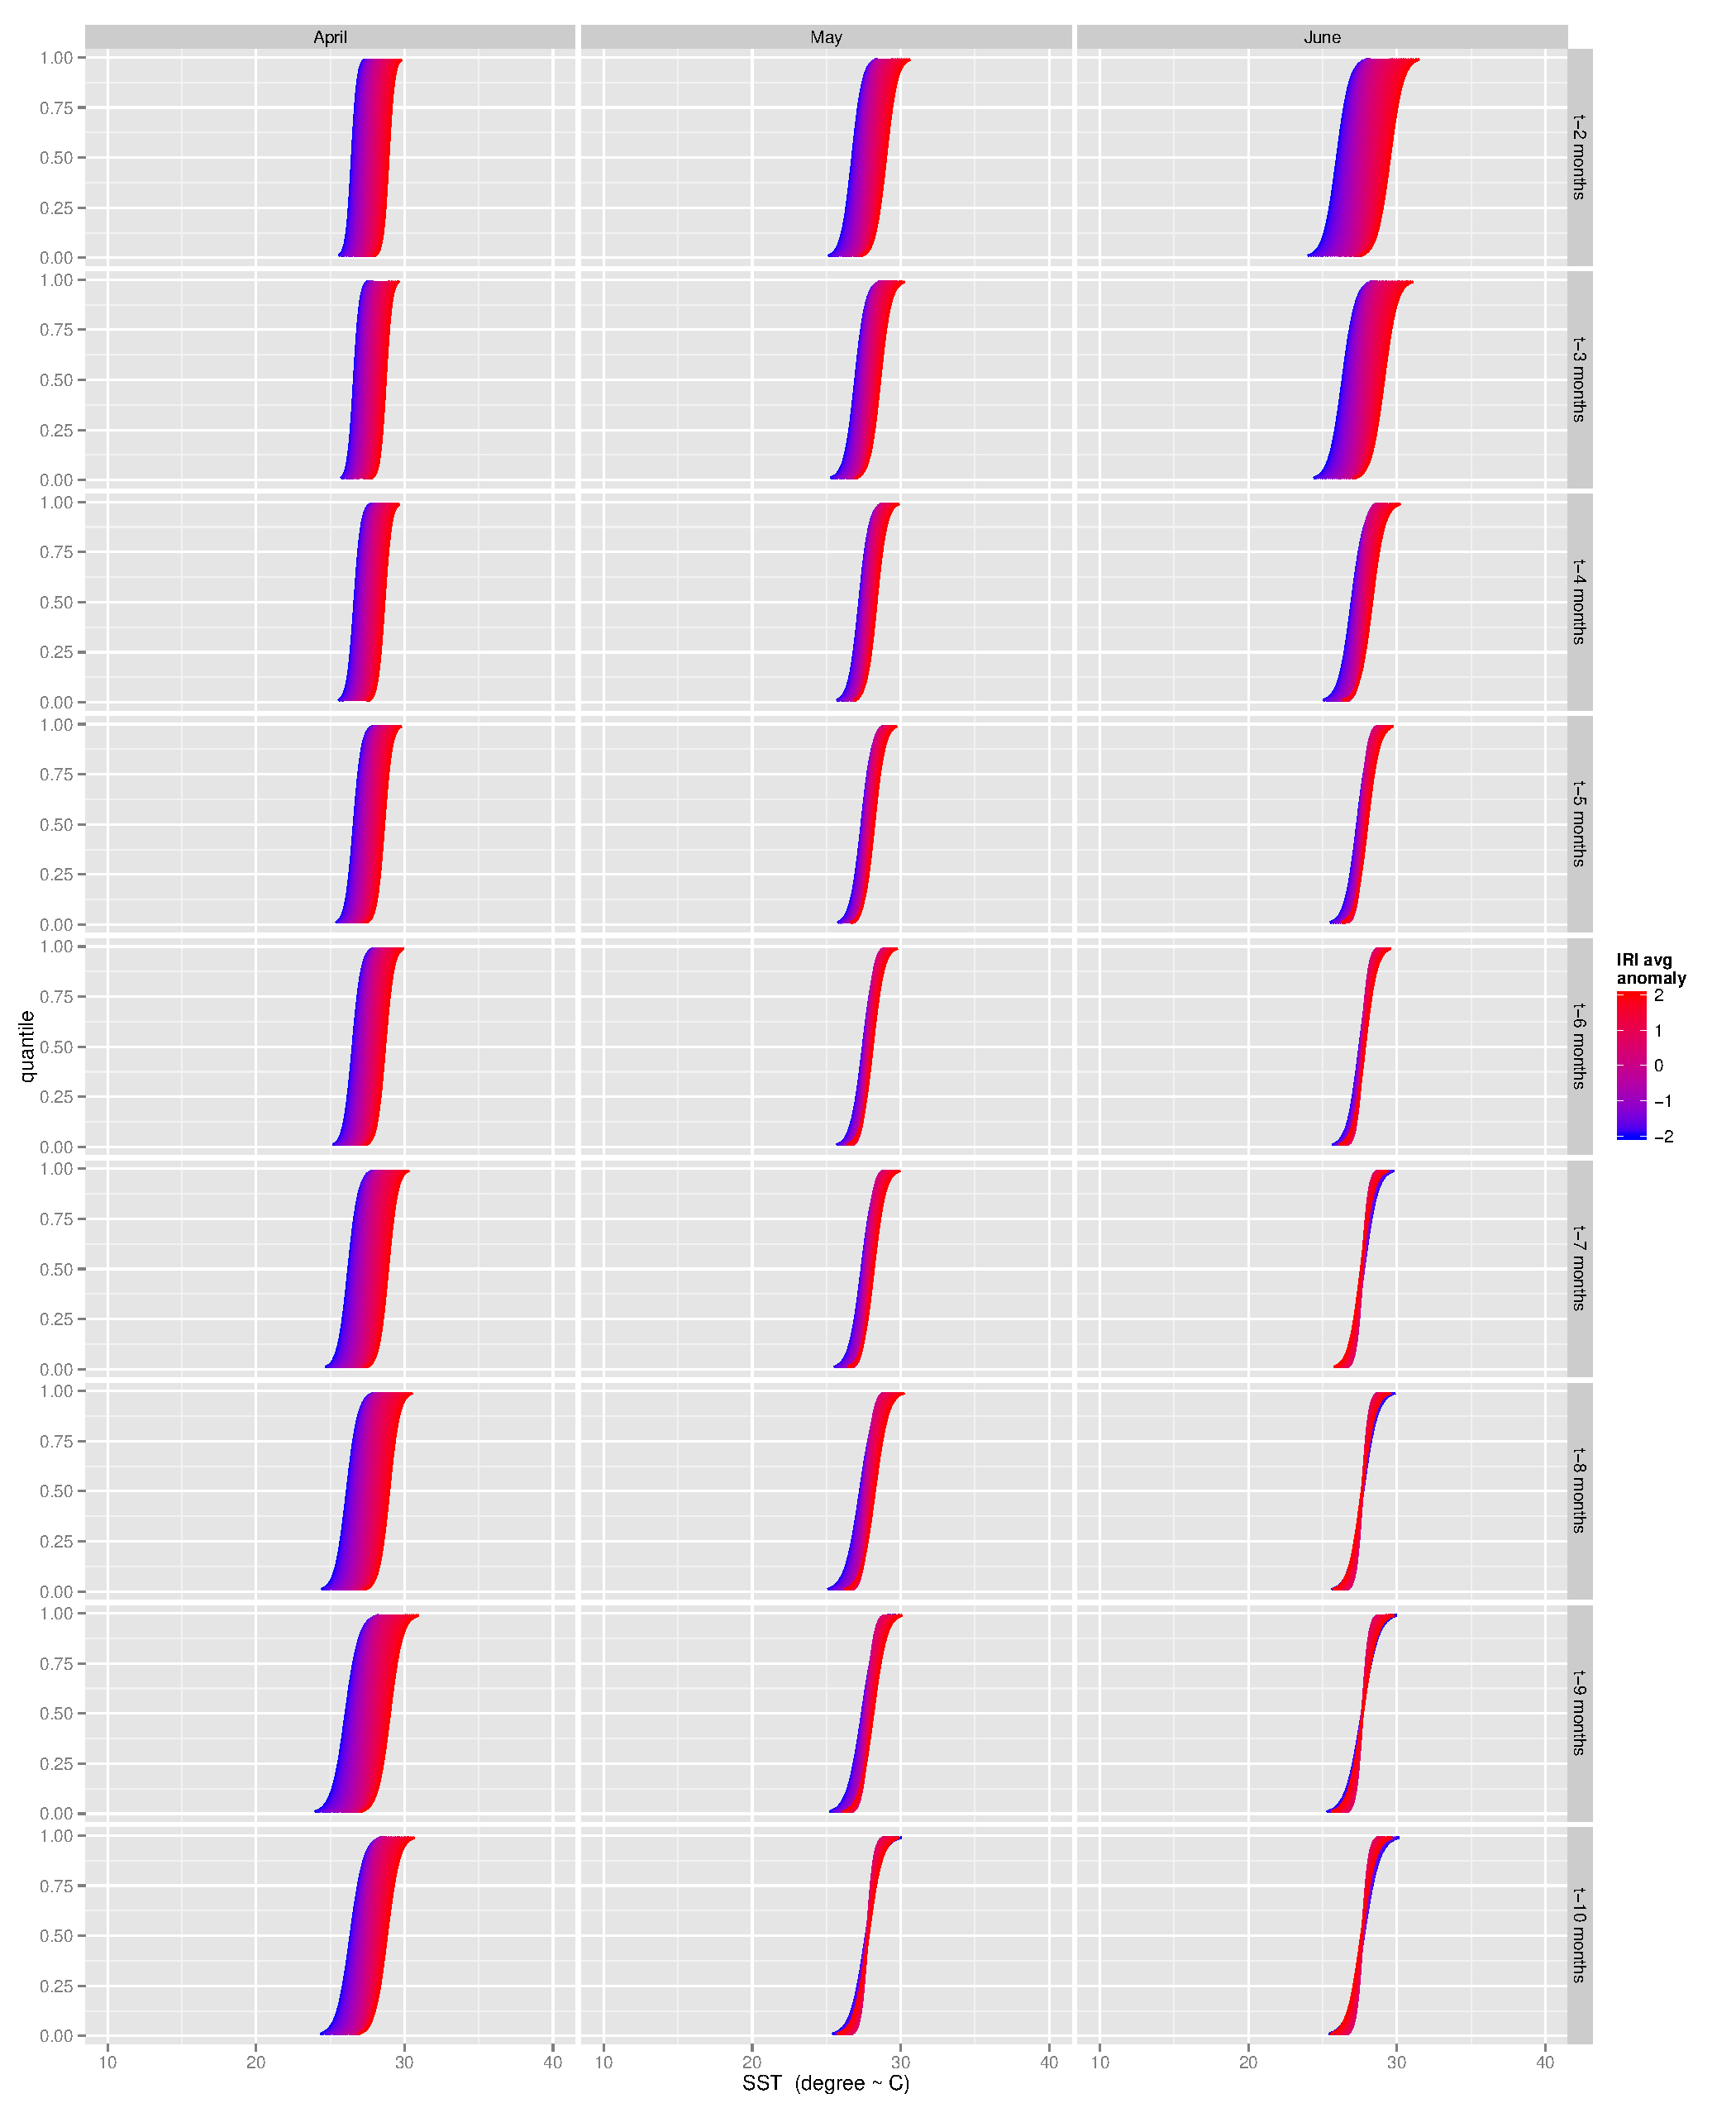
\includegraphics[height=22cm, keepaspectratio]{Pricingfigs/conditionalCDFs04to06TraditionalCDFconfig}
  \caption{Empirical cumulative distribution functions for April through June Ni\~no 3.4 SST conditioned on average IRI ensemble forecasts available for various months. ECDFs are of draws from the posterior predictive distribution of the model specified in equation \ref{eqn:conditionalEstEqn}.}
   \label{fig:conditionalCDFs04to06}
   \end{center}
\end{figure}


\begin{figure}[!htbp]
\begin{center}
  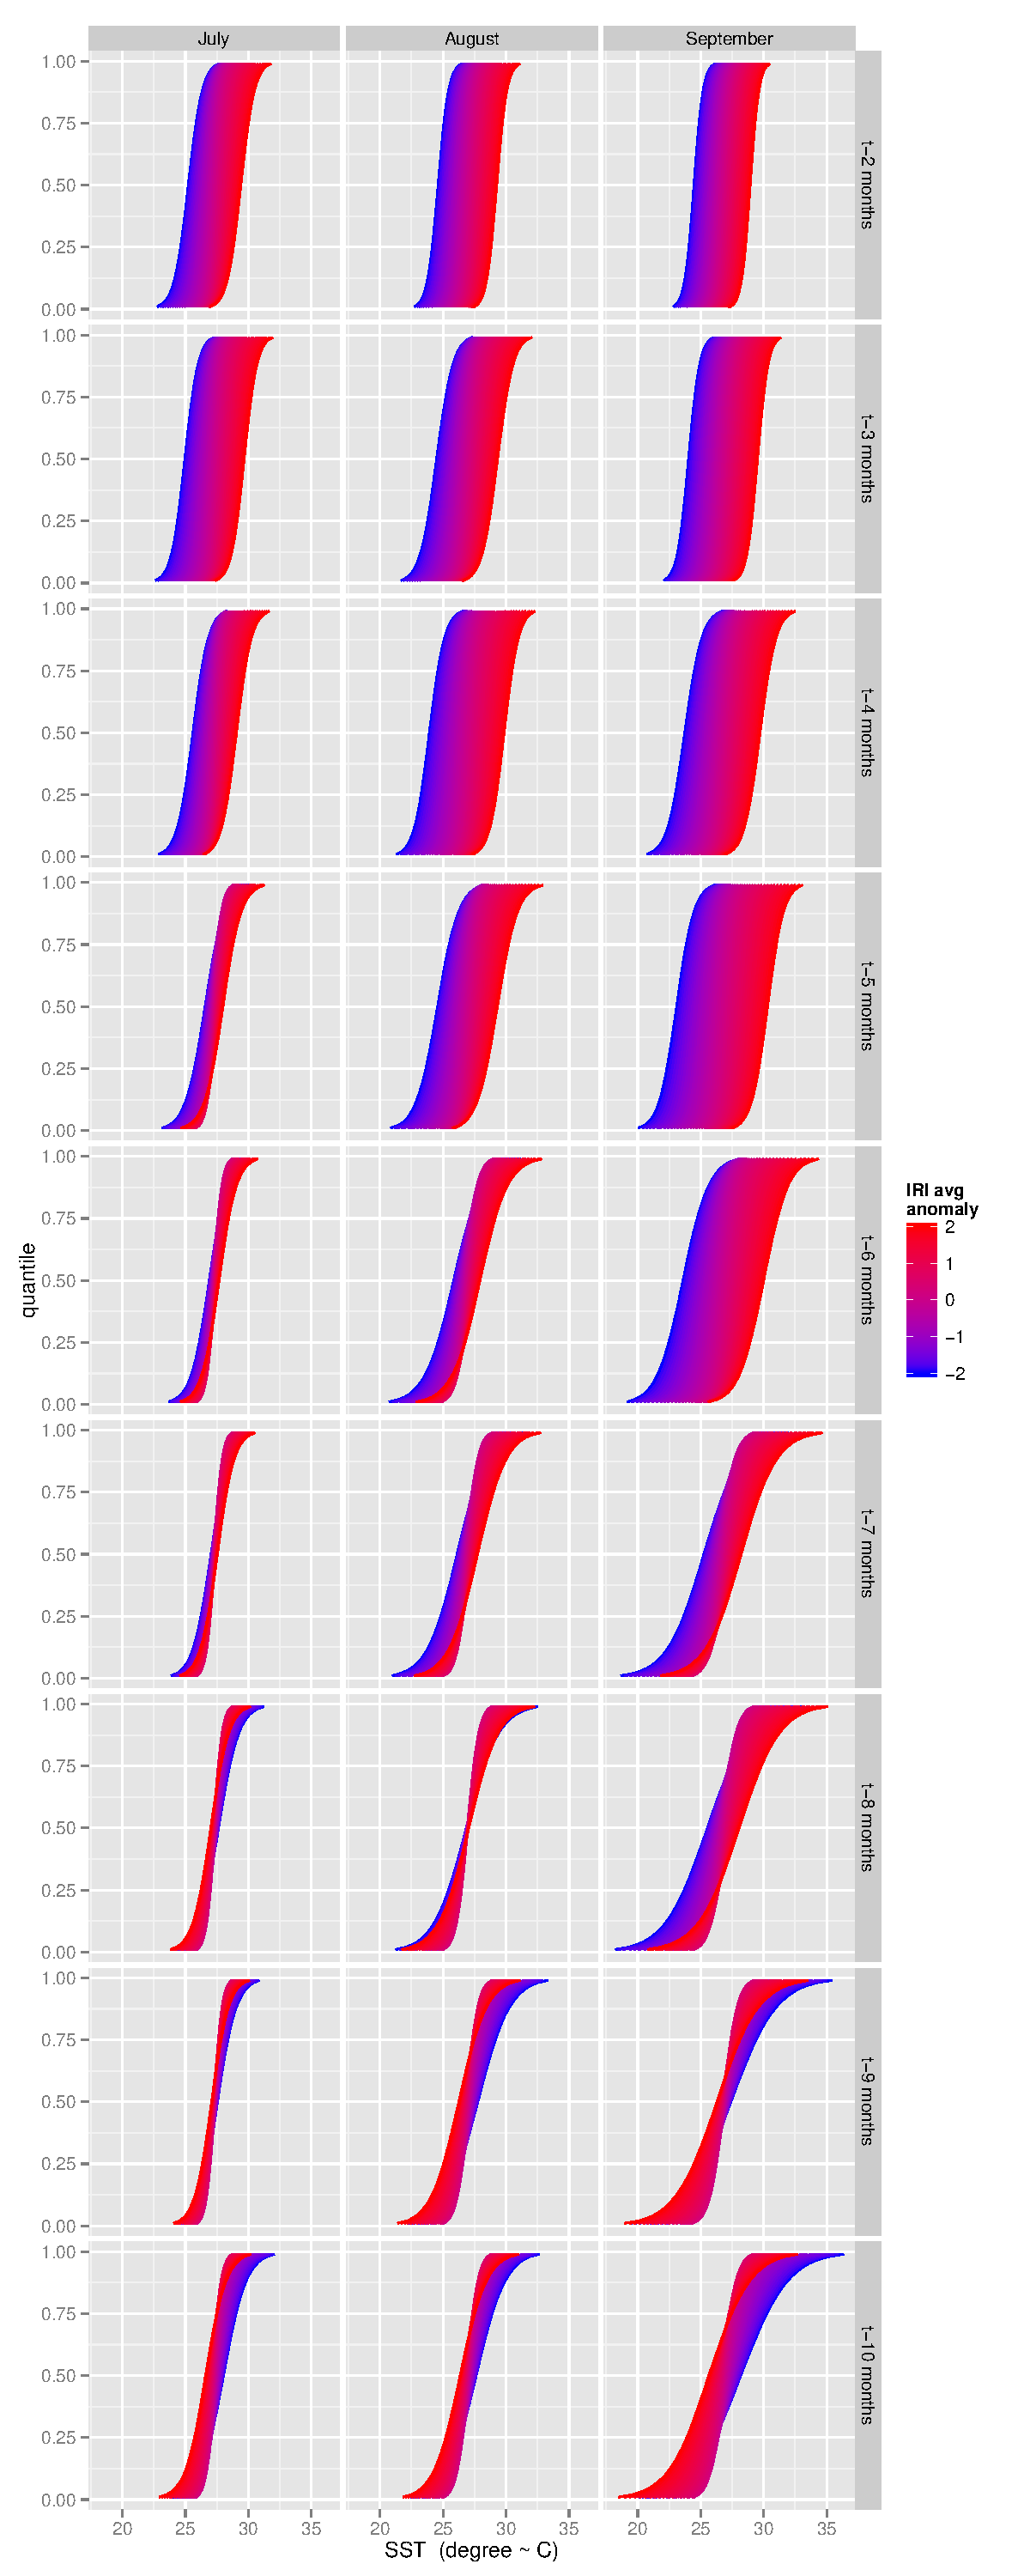
\includegraphics[height=22cm, keepaspectratio]{Pricingfigs/conditionalCDFs07to09TraditionalCDFconfig}
  \caption{Empirical cumulative distribution functions for July through September Ni\~no 3.4 SST conditioned on average IRI ensemble forecasts available for various months. ECDFs are of draws from the posterior predictive distribution of the model specified in equation \ref{eqn:conditionalEstEqn}.}
   \label{fig:conditionalCDFs07to09}
   \end{center}
\end{figure}

\begin{figure}[!htbp]
\begin{center}
  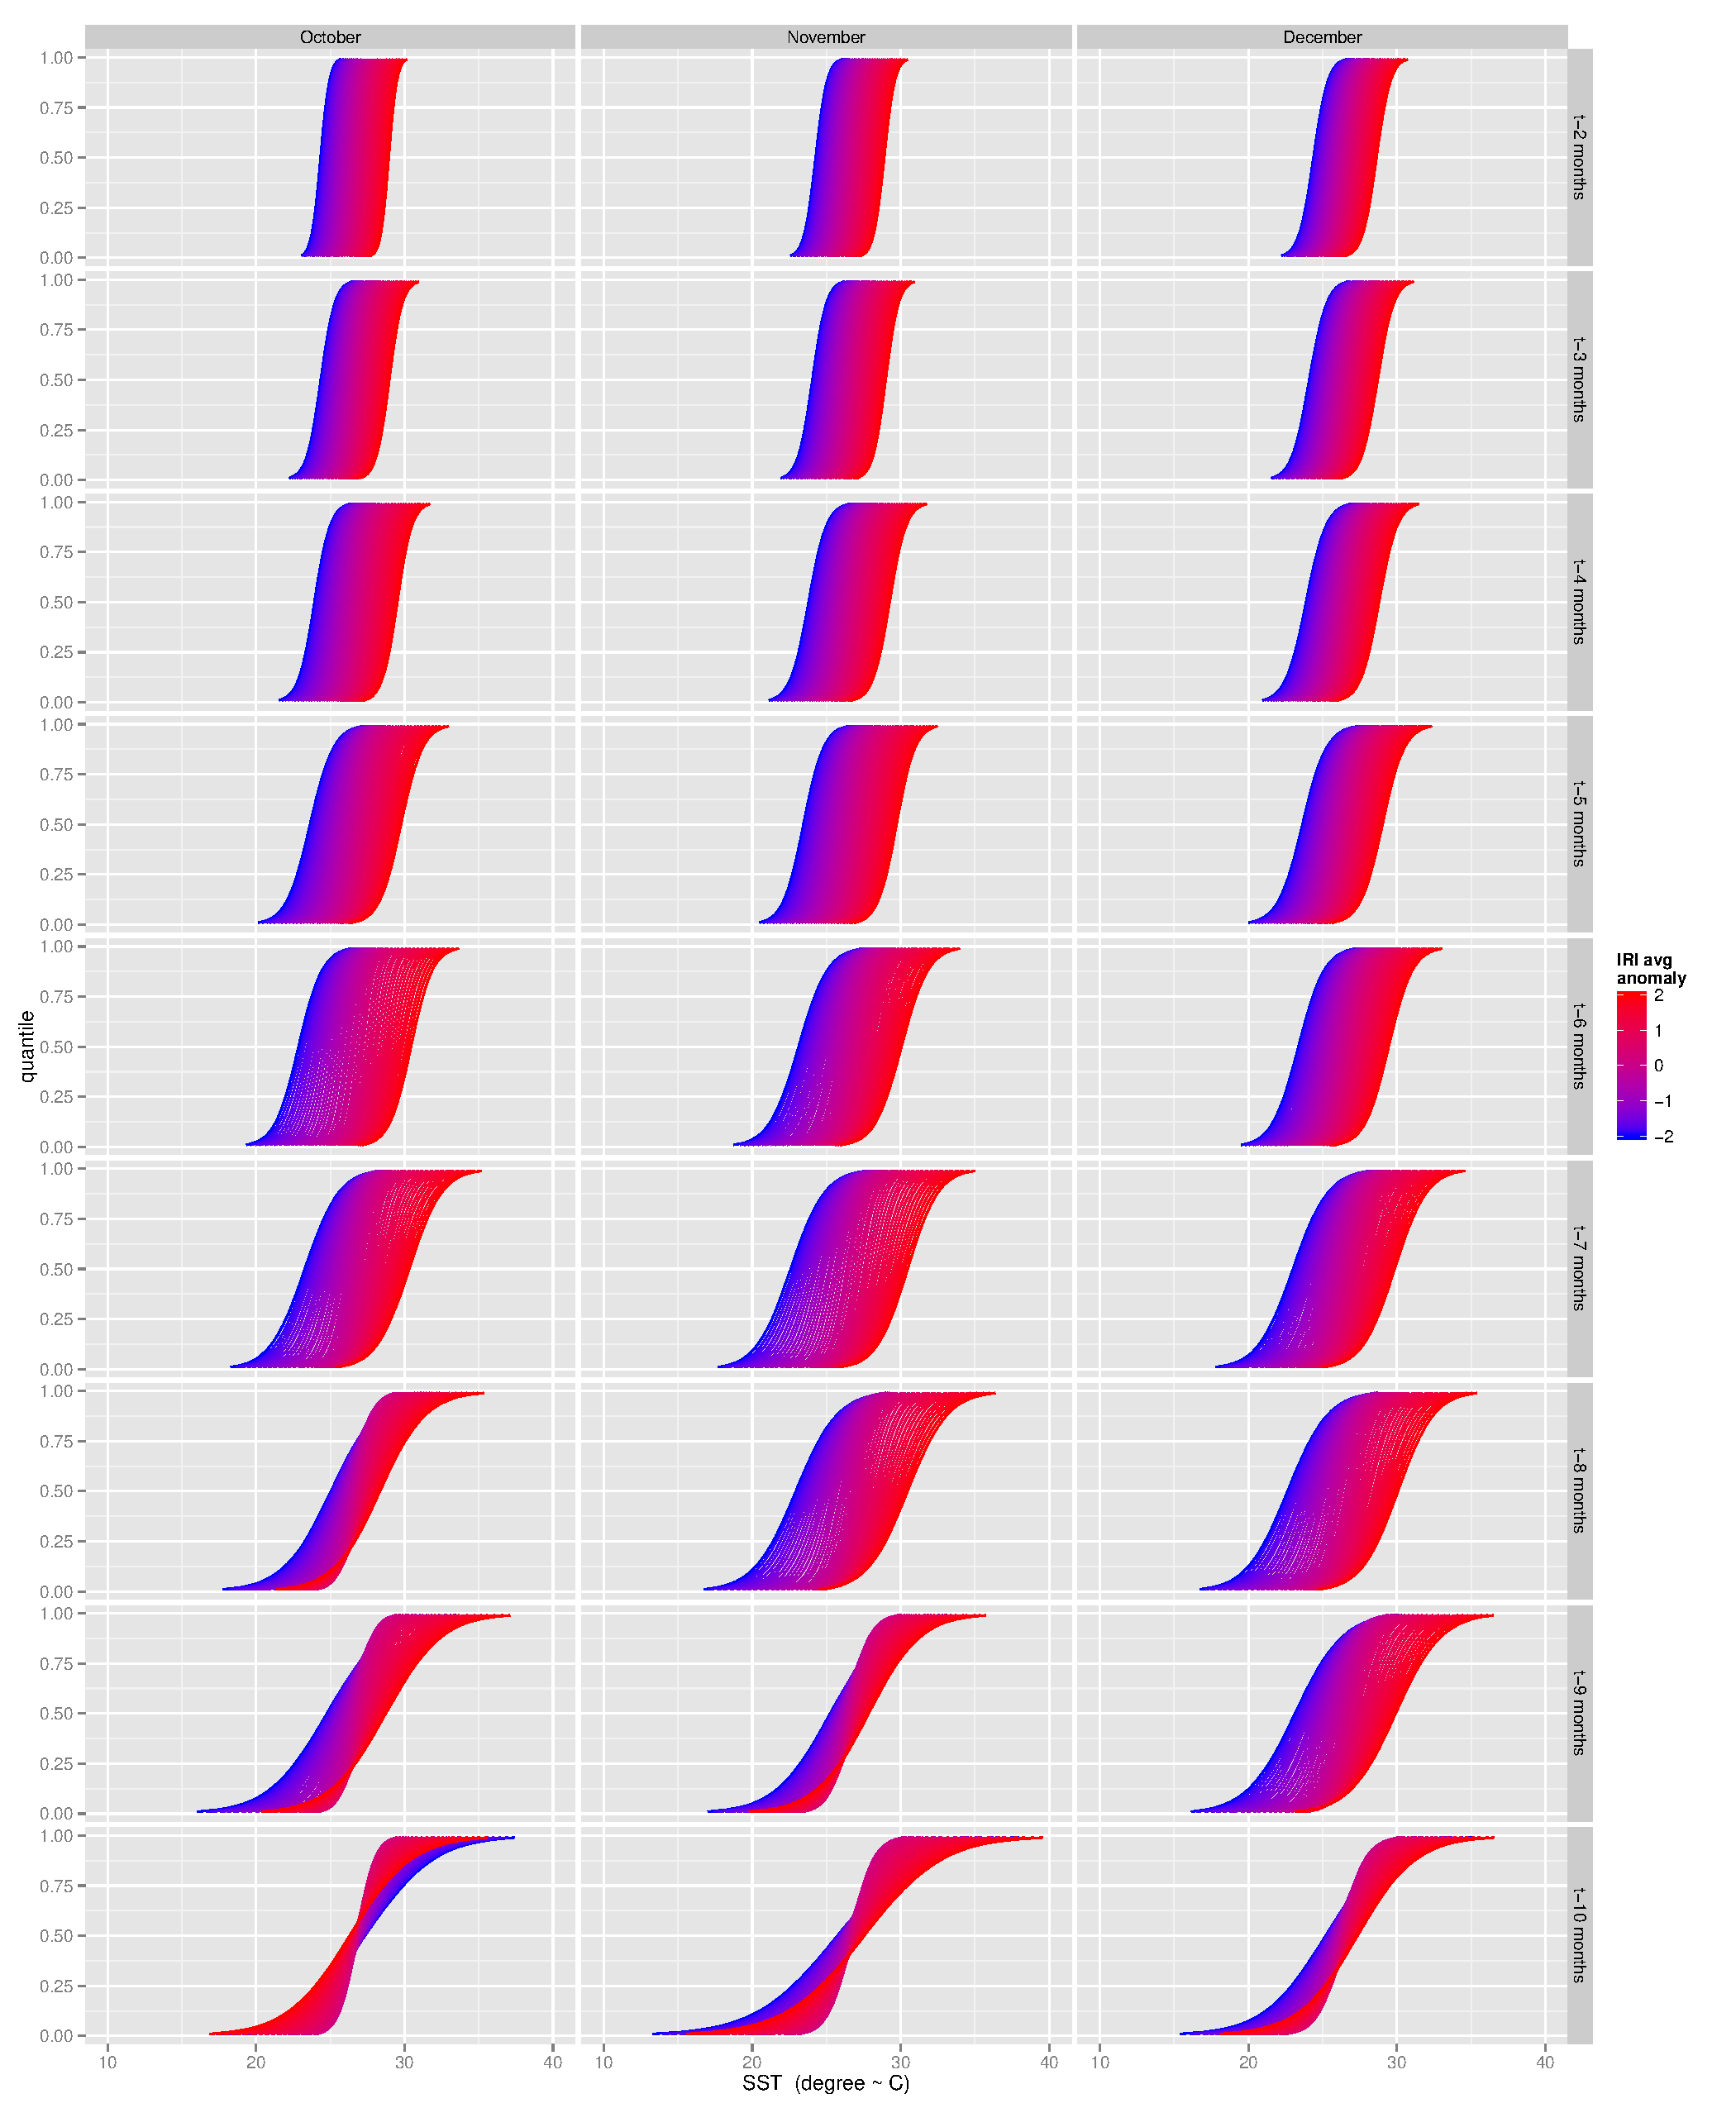
\includegraphics[height=22cm, keepaspectratio]{Pricingfigs/conditionalCDFs10to12TraditionalCDFconfig}
  \caption{Empirical cumulative distribution functions for October through December Ni\~no 3.4 SST conditioned on average IRI ensemble forecasts available for various months. ECDFs are of draws from the posterior predictive distribution of the model specified in equation \ref{eqn:conditionalEstEqn}.}
   \label{fig:conditionalCDFs10to12}
   \end{center}
\end{figure}

\begin{figure}[!htbp]
\begin{center}
  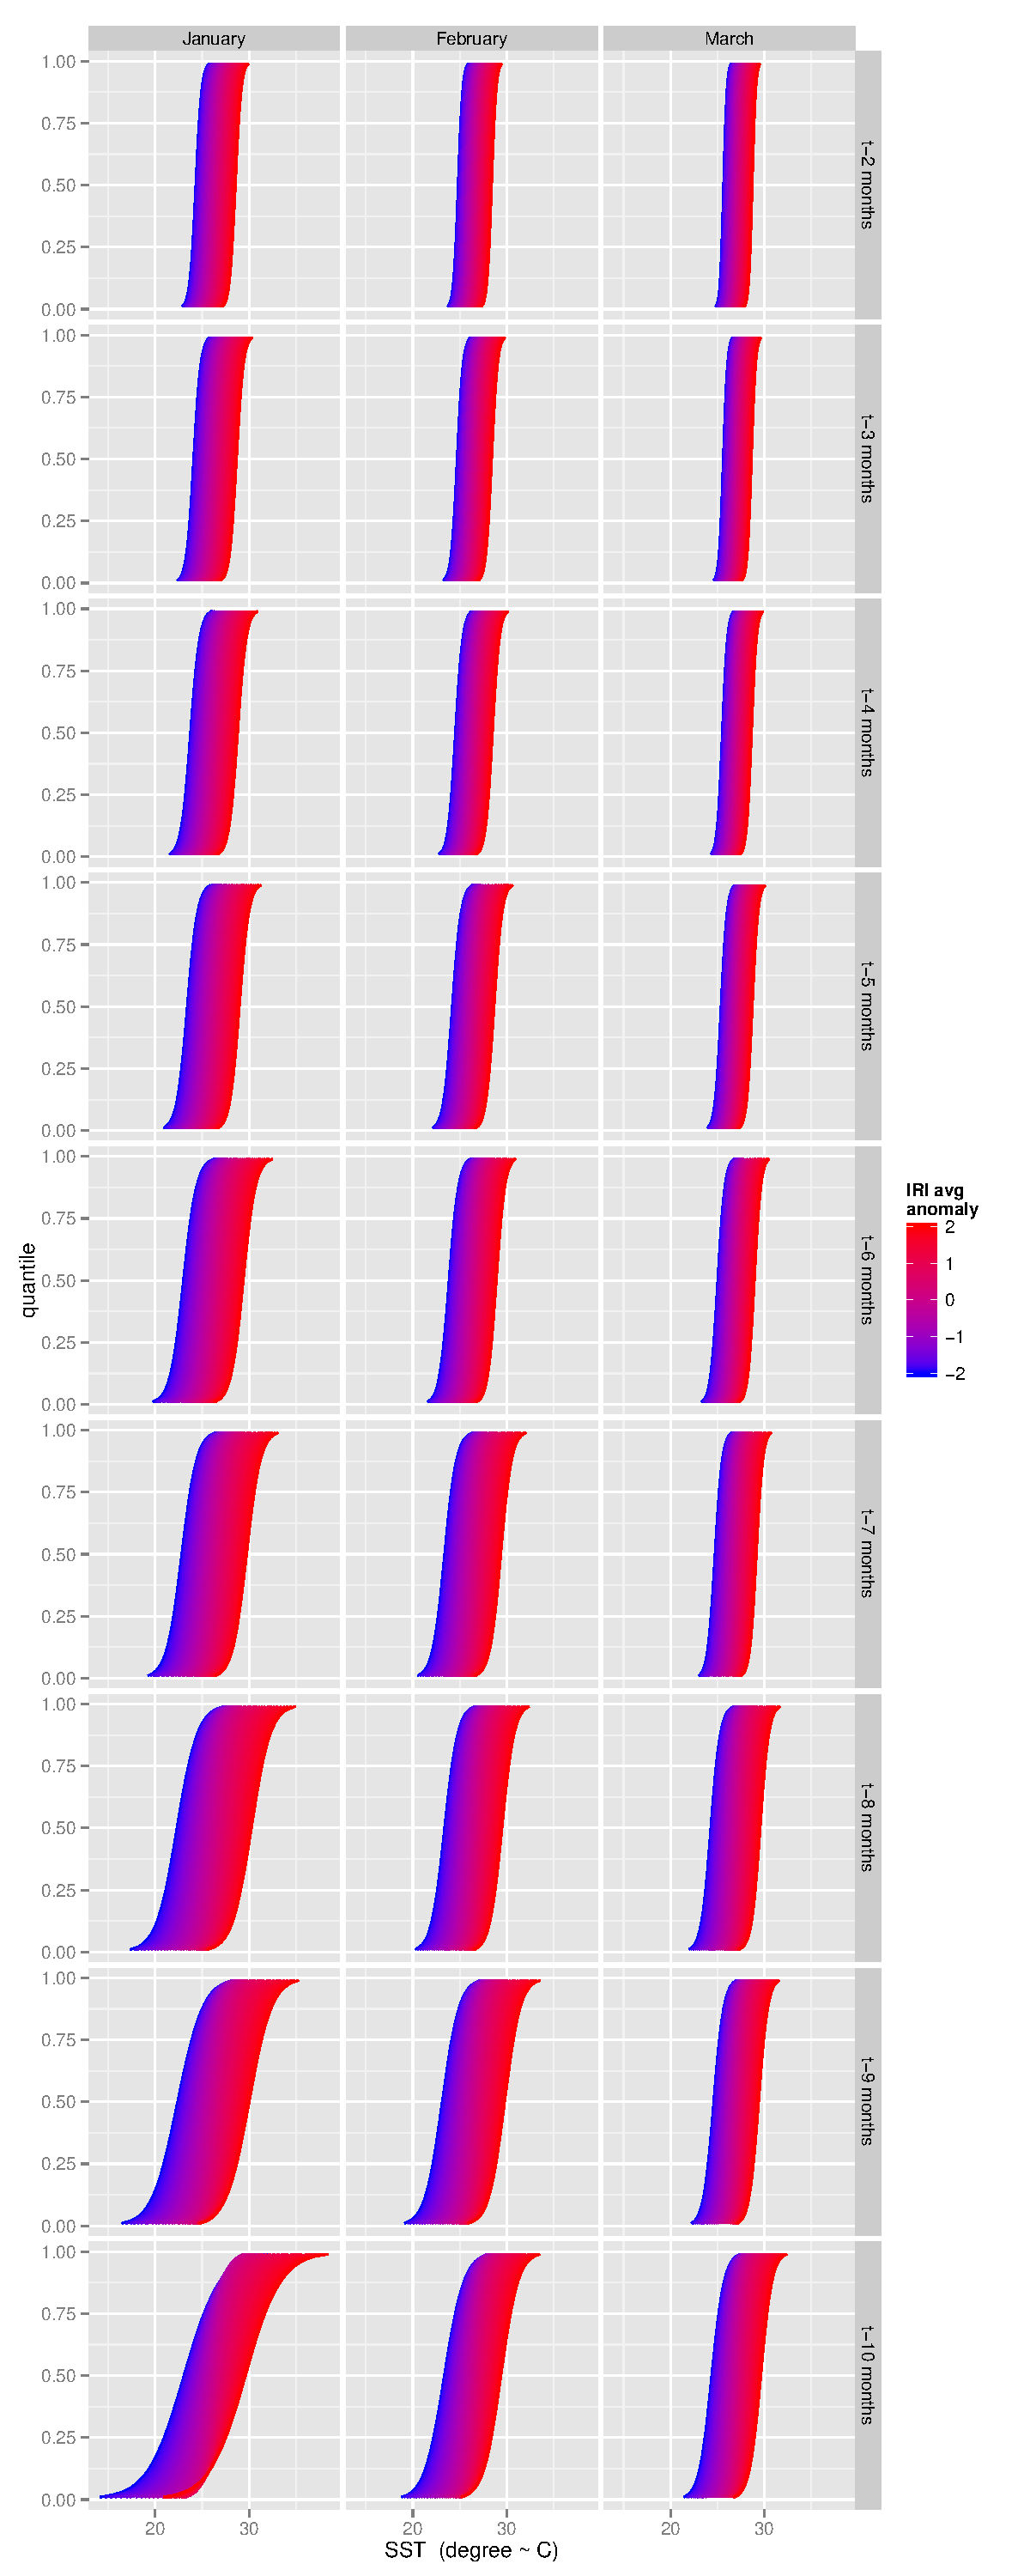
\includegraphics[height=22cm, keepaspectratio]{Pricingfigs/conditionalCDFs01to03TraditionalCDFconfig}
  \caption{Empirical cumulative distribution functions for January through March Ni\~no 3.4 SST conditioned on average IRI ensemble forecasts available for various months. ECDFs are of draws from the posterior predictive distribution of the model specified in equation \ref{eqn:conditionalEstEqn}.}
   \label{fig:conditionalCDFs01to03}
   \end{center}
\end{figure}

The spring predictive barrier is also clear in the figures. In the October column of figure \ref{fig:conditionalCDFs10to12} red and blue lines show substantial overlap for predictions made in February (8 months prior) but that ceases by March.

Notice that most of the ECDFs show their greatest spread along the x-axis when they are furthest out from their target month. This reflects the fact there there are relatively few long-dated extreme forecasts in our sample. The diffuse priors on our parameters results in high uncertainty for simulated outcomes when the sample size is small. The model in equation \ref{eqn:conditionalEstEqn} allows for simulated results that are much higher and lower than any observed SSTs in cases where there are strong but unreliable forecasts.  


% latex table generated in R 3.0.0 by xtable 1.7-1 package
% Tue May  7 21:48:49 2013
\begin{table*}[ht]
\centering \footnotesize
\begin{tabular}{rrrrrrrr}
  \hline
$\mbox{IRI anom}$ & $\mbox{price per USD}$ & $\mbox{E}[\mbox{SST}]$ & $2.5^{\mbox{th}}$ q & $25^{\mbox{th}}$ q & $50^{\mbox{th}}$ q & $75^{\mbox{th}}$ q & $97.5^{\mbox{th}}$ q \\ 
  \hline
-2.00 & 0.80 & 23.93 & 0.00 & 0.66 & 0.96 & 1.00 & 1.00 \\ 
  -1.90 & 0.77 & 24.07 & 0.00 & 0.59 & 0.89 & 1.00 & 1.00 \\ 
  -1.80 & 0.73 & 24.21 & 0.00 & 0.54 & 0.82 & 1.00 & 1.00 \\ 
  -1.70 & 0.68 & 24.35 & 0.00 & 0.47 & 0.75 & 1.00 & 1.00 \\ 
  -1.60 & 0.64 & 24.49 & 0.00 & 0.41 & 0.68 & 0.95 & 1.00 \\ 
  -1.50 & 0.58 & 24.63 & 0.00 & 0.34 & 0.60 & 0.87 & 1.00 \\ 
  -1.40 & 0.53 & 24.77 & 0.00 & 0.28 & 0.54 & 0.79 & 1.00 \\ 
  -1.30 & 0.47 & 24.91 & 0.00 & 0.21 & 0.47 & 0.71 & 1.00 \\ 
  -1.20 & 0.41 & 25.05 & 0.00 & 0.15 & 0.39 & 0.63 & 1.00 \\ 
  -1.10 & 0.35 & 25.19 & 0.00 & 0.08 & 0.32 & 0.55 & 1.00 \\ 
  -1.00 & 0.30 & 25.33 & 0.00 & 0.02 & 0.25 & 0.48 & 0.99 \\ 
  -0.90 & 0.24 & 25.47 & 0.00 & 0.00 & 0.18 & 0.40 & 0.90 \\ 
  -0.80 & 0.19 & 25.60 & 0.00 & 0.00 & 0.11 & 0.33 & 0.81 \\ 
  -0.70 & 0.15 & 25.74 & 0.00 & 0.00 & 0.03 & 0.25 & 0.72 \\ 
  -0.60 & 0.11 & 25.88 & 0.00 & 0.00 & 0.00 & 0.17 & 0.63 \\ 
  -0.50 & 0.08 & 26.02 & 0.00 & 0.00 & 0.00 & 0.10 & 0.55 \\ 
  -0.40 & 0.06 & 26.16 & 0.00 & 0.00 & 0.00 & 0.02 & 0.46 \\ 
  -0.30 & 0.04 & 26.30 & 0.00 & 0.00 & 0.00 & 0.00 & 0.38 \\ 
  -0.20 & 0.02 & 26.44 & 0.00 & 0.00 & 0.00 & 0.00 & 0.31 \\ 
  -0.10 & 0.02 & 26.58 & 0.00 & 0.00 & 0.00 & 0.00 & 0.23 \\ 
  0.00 & 0.01 & 26.72 & 0.00 & 0.00 & 0.00 & 0.00 & 0.16 \\ 
  0.10 & 0.01 & 26.86 & 0.00 & 0.00 & 0.00 & 0.00 & 0.08 \\ 
  0.20 & 0.00 & 26.99 & 0.00 & 0.00 & 0.00 & 0.00 & 0.01 \\ 
  0.30 & 0.00 & 27.14 & 0.00 & 0.00 & 0.00 & 0.00 & 0.00 \\ 
  0.40 & 0.00 & 27.27 & 0.00 & 0.00 & 0.00 & 0.00 & 0.00 \\ 
  0.50 & 0.00 & 27.41 & 0.00 & 0.00 & 0.00 & 0.00 & 0.00 \\ 
  0.60 & 0.00 & 27.55 & 0.00 & 0.00 & 0.00 & 0.00 & 0.00 \\ 
  0.70 & 0.00 & 27.69 & 0.00 & 0.00 & 0.00 & 0.00 & 0.00 \\ 
  0.80 & 0.00 & 27.83 & 0.00 & 0.00 & 0.00 & 0.00 & 0.00 \\ 
  0.90 & 0.00 & 27.97 & 0.00 & 0.00 & 0.00 & 0.00 & 0.00 \\ 
  1.00 & 0.00 & 28.11 & 0.00 & 0.00 & 0.00 & 0.00 & 0.00 \\ 
  1.10 & 0.00 & 28.24 & 0.00 & 0.00 & 0.00 & 0.00 & 0.00 \\ 
  1.20 & 0.00 & 28.38 & 0.00 & 0.00 & 0.00 & 0.00 & 0.00 \\ 
  1.30 & 0.00 & 28.53 & 0.00 & 0.00 & 0.00 & 0.00 & 0.00 \\ 
  1.40 & 0.00 & 28.67 & 0.00 & 0.00 & 0.00 & 0.00 & 0.00 \\ 
  1.50 & 0.00 & 28.80 & 0.00 & 0.00 & 0.00 & 0.00 & 0.00 \\ 
  1.60 & 0.00 & 28.95 & 0.00 & 0.00 & 0.00 & 0.00 & 0.00 \\ 
  1.70 & 0.00 & 29.08 & 0.00 & 0.00 & 0.00 & 0.00 & 0.00 \\ 
  1.80 & 0.00 & 29.23 & 0.00 & 0.00 & 0.00 & 0.00 & 0.00 \\ 
  1.90 & 0.00 & 29.36 & 0.00 & 0.00 & 0.00 & 0.00 & 0.00 \\ 
  2.00 & 0.00 & 29.51 & 0.00 & 0.00 & 0.00 & 0.00 & 0.00 \\ 
   \hline
\end{tabular}
\caption[Put option prices for October Ni\~no 3.4 SST conditioned on IRI ensemble forecasts released in June]{Put option prices for October Ni\~no 3.4 SST conditioned on IRI ensemble forecasts released in June} 
\label{tab:pricesOctSub}
\end{table*}


Table \ref{tab:pricesOctSub}, translates simulation results into pricing for October La Ni\~na protection (put options on October SST) conditioned on June forecasts using the payout function discussed above. Notice that June is well within the spring predictive barrier so forecasts of negative SST anomalies greatly increase the expected value of La Ni\~na protection. The full conditional pricing tables for all months, covering both El Ni\~no and La Ni\~na, are available [ONLINE].

We have also provided a price path for La Ni\~na protection during the 2010 ENSO season, which ultimately registered a negative anomaly of -1.52 degrees. In figure \ref{fig:pricesOctober2010} all but the most conservative pricing guideline suggests that La Ni\~na protection has very little expected value prior to the spring predictive barrier. (The most conservative pricing guideline in this case is the pricing guideline that follows the 97.5th percentile of the distribution of simulated payouts given then prevailing forecasts.) By April (t-6 months), figure \ref{fig:predOctober2010} indicates that IRI forecasts were suggesting a moderate La Ni\~na season. Given the growing predictive power of those forecasts after the spring predictive barrier, La Ni\~na coverage begins climbing in value from the standpoint of someone pricing according to the 75th percentile of simulated values. By June, forecasts have fallen further while their informational value has steadily risen, giving La Ni\~na protection a positive value according to less conservative pricing benchmarks. By August, most pricing benchmarks actually suggests a value for La Ni\~na coverage that is actually higher than the payout resulting from October 2010's measured SSTs.

\begin{figure*}[!htbp]
  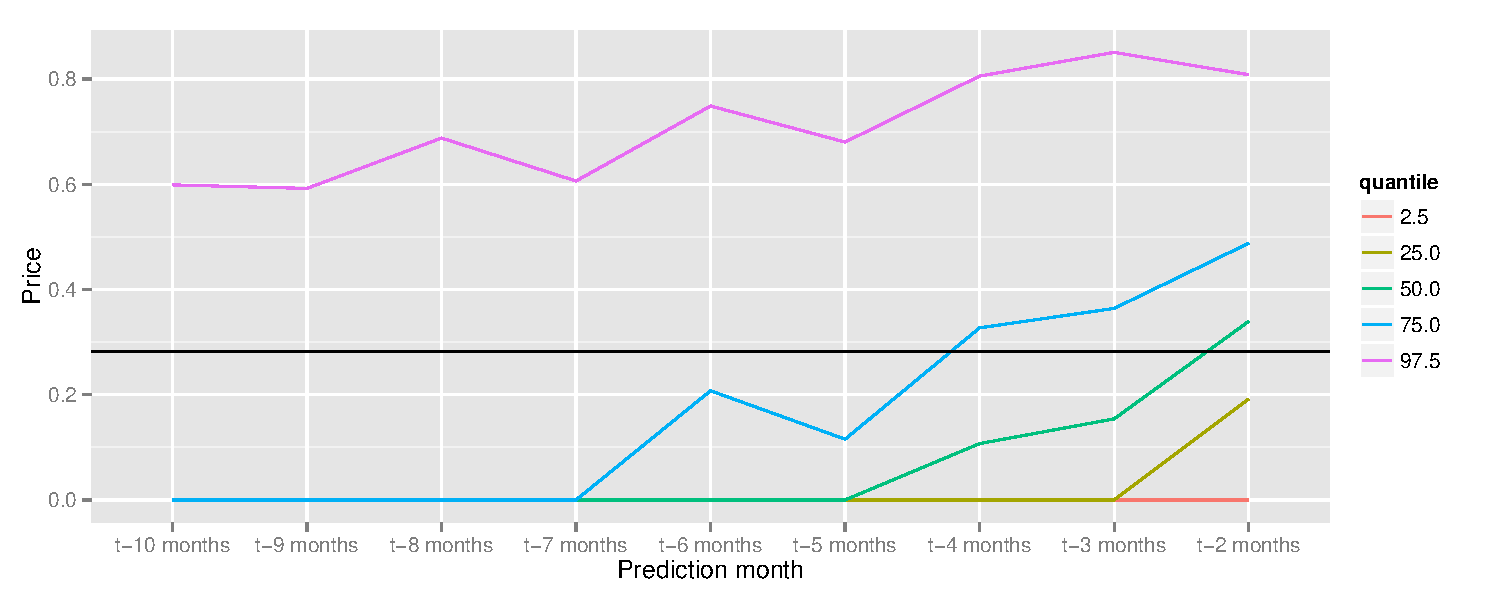
\includegraphics[width=\linewidth]{Pricingfigs/pricesOctober2010}
  \caption{Prices by quantile for October 2010 La Ni\~na protection conditioned on available forecasts. Payout for actual October 2010 Ni\~no 3.4 SST in black.}
   \label{fig:pricesOctober2010}
\end{figure*}

\begin{figure*}[!htbp]
  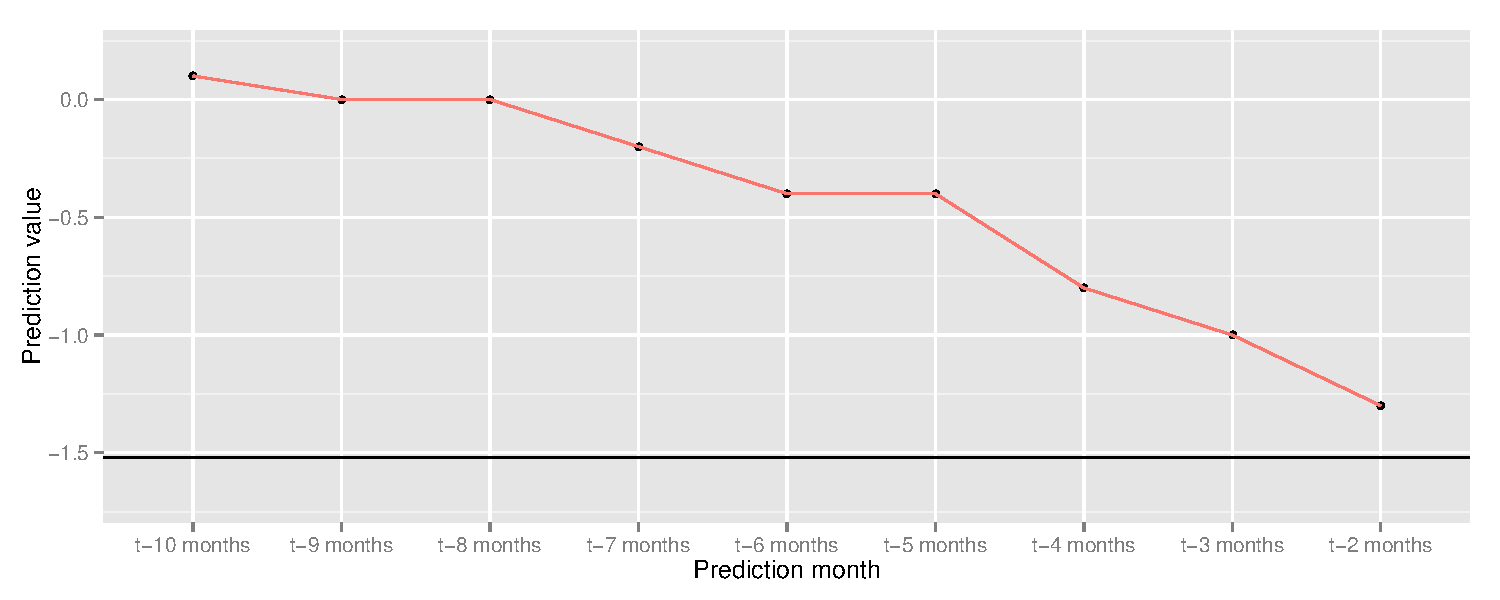
\includegraphics[width=\linewidth]{Pricingfigs/predOctober2010}
  \caption{IRI average anomaly forecast for October 2010. Actual October 2010 Ni\~no 3.4 SST anomaly in black.}
   \label{fig:predOctober2010}
\end{figure*}



\subsubsection{Result 1} 
stochastic catalog

\subsubsection{Result 2}
Information is more important at some points than others



\section{Application}
\subsection{Key changes to make this operational}
The prices in table \ref{tab:pricesOctSub} and [ONLINE] only reflect the underlying risk of the index. In actual transactions, these pure risk prices will generally be:
\begin{itemize}
\item adjusted (downward) to reflect the time value of the premium paid by hedgers;
\item subjected to some margining\footnote{Margining refers to the process of setting aside collateral on financial trades. On exchange-traded derivatives there are clear, predictable rules for how much money must be set aside as collateral in a \emph{margin account} as the trade's settlement index changes over time.} rules, when applicable; and
\item adjusted (upward) to allow for some reasonable expected profit for speculators.
\end{itemize}

\subsection{Understanding informational and monetary gains from better forecasts}

\subsection{Remove best forecast and compare pricing with and without it. What is the earning opportunity?}

\subsection{Alternatively: application of finding natural swaps}







\section{Conclusion}
Introduced a important new concept for risk management - traded direct climate markets

and walked though some of the early steps in launching that market

steps that are broadly applicable to other such risks - particularly the teleconnection indexes that may be launched in years to come.

Next steps - we've talked about traded risk markets but which - options swaps and cat bonds

How can NMS support the use of these - licensing








\subsection{Key results summary}

\subsubsection{Distributional properties – several assumptions seem to work}

\paragraph{Normality assumption works well (and may have analytical benefits?)}

\subsubsection{Information changes significantly and so motivates dynamic pricing}

\paragraph{Inflection points and critical information}

\paragraph{Identifying the magnitude of uncertainty and its pricing implications}

\paragraph{IRI ensemble forecast can provide foundation for baseline}

\subsection{Other necessary conditions for traded market}

\subsection{Positive externalities}

\subsubsection{Better climate models (O.J. futures example)}

\subsubsection{Should government finance the startup?}

\bibliographystyle{dcu}
\bibliography{References/references}

\end{document}
